\section{Introduction}

\section{The Herschel-ATLAS}
\label{sec:The Herschel-ATLAS}

The \textit{Herschel} Astrophysical Terahertz Large Area Survey (H-ATLAS; \citealt{Eales_2010}) was the largest open-time sub-mm survey carried out with the \textit{Herschel Space Observatory}. The survey was observed across five photometric bands using two instruments onboard \textit{Herschel}: the Photodetector Array Camera (PACS, \citealt{Poglitsch_2010}) at 100 and 160\,\micron, and the Spectral and Photometric Imaging Receiver (SPIRE, \citealt{Griffin_2010}) at 250, 350 and 500\,\micron\ {\color{red}Repeated from the introduction}. Compared to the first SMGs detected using SCUBA at 850\,\micron (\citealt{Smail_1997}; \citealt{Barger_1998}; \citealt{Hughes_1998}), the PACS and SPIRE wavebands span the peak of the infrared spectrum for low redshift (z < 1) galaxies and thus their intrinsic brightness at the SPIRE wavelengths makes their detection in the thousands possible over large sky fields. The main scientific goal of the survey was to estimate the dust masses and dust obscured star formation rates for thousands of nearby galaxies over a large area of sky, however, the surprising sensitivity of \textit{Herschel} and the negative k-correction observed at the SPIRE wavelengths (\citealt{Blain_1993}) means that a substantial fraction of sources were observed at higher redshifts, with a median of z $\sim$ 1. The catalogues of the survey, as detailed below, includes sources with redshifts up to $\sim$ 6 (\citealt{Amblard_2010}; \citealt{Lapi_2011}; \citealt{Fudamoto_2017}; \citealt{Zavala_2018}).

The complete survey covers $\sim$\,660\,$\deg^2$, split into three regions located to avoid emission from Galactic dust and to utilize complementary spectroscopic surveys including the Sloan Digital Sky Survey (SDSS, \citealt{York_2000}), the 2df Galaxy Redshift Survey (2dfGRS, \citealt{Colless_2001}) and the Galaxy and Mass Assembly (GAMA, \citealt{Driver_2009}). The three areas are: The North Galactic Pole (NGP) region covering $\sim$\,180\,$\deg^2$ of the northern sky, centered at R.A 13$^{h}$18$^{m}$ and declination +29$^{\circ}$13' (J2000); three equatorial fields, located at approximately R.A 9$^{h}$, 12$^{h}$ and 15$^{h}$ coinciding with the GAMA survey (henceforth named GAMA9, GAMA12 and GAMA15 fields), each with an area of approximately 54\,$\deg^2$; and the South Galactic Pole (SGP) region, centered at R.A 0$^{h}$6$^{m}$ and declination -32$^{\circ}$44' (J2000) with an area of $\sim$ 318\,$\deg^2$. 

\subsection{Detecting Submillimeter Sources on Herschel Images}
\label{sec:Detecting Submillimeter Sources on Herschel Images}

Given the poor angular resolution of \textit{Herschel} (ranging between 5" and 37" from 70\,\micron to 500\,\micron) the sub-mm images it produces contain two main types of noise: instrumental noise, which is not typically correlated between pixels, and confusion noise which is highly correlated between pixels, most of its contribution coming from the blending together of faint sources. Source confusion is of particular importance to sub-mm surveys where the angular resolution is of the order 1000 times worse than at optical wavelengths. The result of combining instrumental noise with confusion noise is that almost all sources in the \textit{Herschel} images are unresolved and the optimum filter for detecting these unresolved sources is no longer the point spread function (PSF). Considering a \textit{Herschel} map in which there is only one source of noise: an image with instrumental noise but no confusion noise (i.e. there is only one point source and no fainter, confusing sources), the optimal detection of this source is obtained by convolving the image with the PSF of the instrument. On the other hand, a map with no instrumental noise, but many confused point sources would be optimally detected with its best signal to noise ratio (SNR) by taking the Fourier transform of the image, dividing by the Fourier transform of the PSF and taking the inverse Fourier transform to obtain a perfect deconvolution of the original map (\citealt{Valiante_2016}). For images that have a variable ratio of instrumental to confusion noise like the \textit{Herschel} images of H-ATLAS, \citealt{Chapin_2011} showed that a convolving function or "matched filter" can be calculated to provide the maximum SNR for an unresolved source.

To detect H-ATLAS sources from the 250\,\micron maps using a matched filter (the 250\,\micron band is the most sensitive of the SPIRE bands and given the lower sensitivity of the PACS instrument, all sources detected on the PACS images would also be detected on the SPIRE 250\,\micron image), \citealt{Maddox_2020} developed a source detection algorithm called the Multi-band Algorithm for Source Detection and eXtraction (\texttt{MADX}). The \texttt{MADX} algorithm works in the following way. Firstly, Galactic dust emission is removed from the images using \texttt{Nebuliser}, a program that removes large scale variations in the background of an image, then the images are convolved with the matched filter. The corresponding variance map is created by convolving the map of variance in instrumental noise with the matched filter and adding the confusion noise. It is from this map that the SNR of a detected source is determined. The same process is repeated with the 350 and 500\,\micron maps and interpolated to the same pixel scale as the 250\,\micron maps. The detection map used to extract sources is then generated from a weighted sum of the three SPIRE maps, however, due to the smaller PSF at 250\,\micron, which leads to more accurate positions and an increased number of detected sources, zero weighting is given to the 350 and 500\,\micron images. This has the effect of making the detection map the same as the 250\micron map.

Sources are identified by peak values > 2.5$\sigma$ in the filtered detection map and their positions are estimated by fitting a Gaussian to the nearest pixels surrounding the location of the peak. The source is extracted in the other \textit{Herschel} wavebands at the 250\,\micron position. Due to the high levels of confusion and high source density on the SPIRE maps, the flux density estimates in each band can be biased by blending with other sources. The \texttt{MADX} algorithm negates some of this problem by ordering the sources by their flux density and iteratively fitting and removing a point source from the position of each source, starting with the brightest. The new estimates of the flux densities are then not influenced by contamination from brighter sources. The catalogue of point sources provided by the H-ATLAS project come from the extraction of point sources using \texttt{MADX} applied to the SPIRE images of the NGP, SGP and GAMA fields. The final catalogues are reduced to those sources with SNR > 4 in any of the SPIRE bands. While this detection method suggests that we may miss sources that are faint at 250\,\micron but bright at 350 or 500\,\micron due to the weighting of the three images, cataloguing all sources with SNR > 4 in any of the SPIRE bands means that the catalogues are reasonably complete in all bands. The completeness of the sub-mm catalogues, as a function of the measured flux density of a given source as estimated by simulations run by \citealt{Valiante_2016}, is illustrated in Figure \ref{fig:submm_completeness}.

\begin{figure}
    \centering
	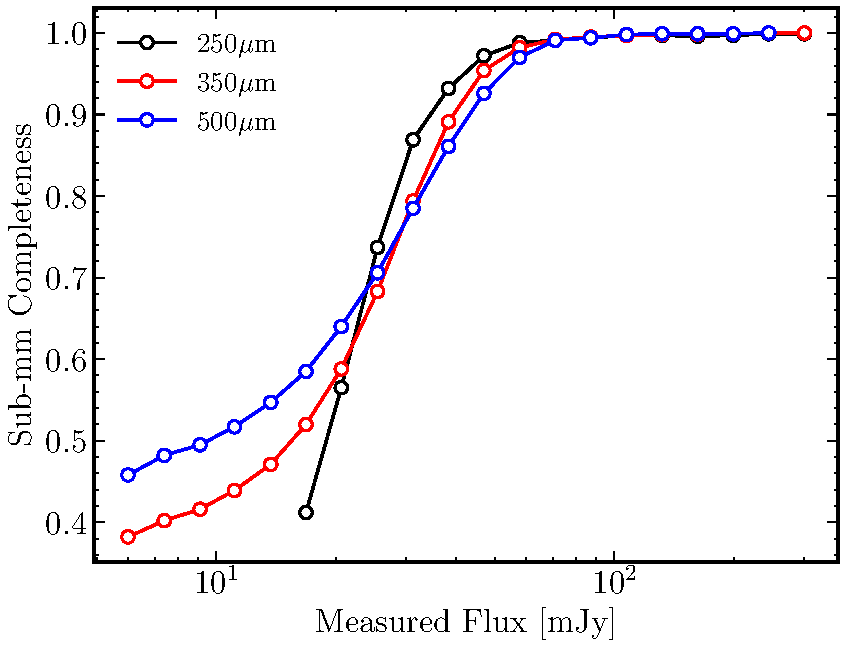
\includegraphics[width=0.75\columnwidth]{Figures/submm_completeness.pdf}
	\caption{The completeness of the H-ATLAS Data Release I catalogues of sub-mm sources, as a function of the measured flux density at 250\,\micron (black) 350\,\micron (red) and 500\,\micron (blue). This figure is recreated from Figure 21 in \citealt{Valiante_2016}.}
	\label{fig:submm_completeness}
\end{figure}

\subsection{Data Releases of the H-ATLAS}
\label{sec:Data Releases of the H-ATLAS}

The first public data release (DR1) of H-ATLAS covered the three equatorial GAMA fields, which span approximately 25\% of the total survey area. These fields benefit from multiwavelength coverage from GAMA, SDSS, 2dF, the Galaxy Evolution Explorer (GALEX, \citealt{Martin_2005}), the UKIRT Infrared Deep Sky Survey -- Large Area Survey (UKIDSS-LAS, \citealt{Lawrence_2007}), the Wide-field Infrared Survery Explorer (WISE, \citealt{Wright_2010}), the VISTA Kilo-degree Infrared Galaxy survey (VIKING, \citealt{Edge_2013}) and the Kilo-Degree Survey (KiDS, \citealt{deJong_2013}). 

Sub-mm sources are provided in DR1 if they are detected above the 2.5$\sigma$ detection limit on the 250\,\micron map and have measured flux densities greater than the 4$\sigma$ flux density limits in one of the three SPIRE bands (29.6\,mJy, 37.6\,mJy or 40.8mJy at 250, 350 and 500\,\micron). Across the three fields there are a total of 113,995, 46,209 and 11,011 sources detected at > 4$\sigma$ at 250, 350 and 500\,\micron as well as detections for 4,650 and 5,685 sources at > 3$\sigma$ at 100 and 160\,\micron (\citealt{Valiante_2016}). Following the release of the sub-mm sources detected in the GAMA fields, \citealt{Bourne_2016} used the Likelihood Ratio (LR, \citealt{Sutherland_1992}; \citealt{Ciliegi_2003}) method (see also Section \ref{sec:The Likelihood Ratio Method}) to identify potential optical counterparts from SDSS to the 113,995 sources with SNR$_{250}$ > 4. Sources with SNR$_{250}$ < 4 that were detected by their 350 or 500\,\micron flux densities were omitted from the matching since these sources have sub-mm colours suggesting a high redshift, and are the most likely sources to be misidentified by SDSS due to the increased probability of chance alignments or gravitational lensing along the line of sight (\citealt{Negrello_2010}; \citealt{Pearson_2013}; \citealt{Bourne_2014}). \citealt{Bourne_2016} identified optical counterparts within 10" of 44,385 (39\%) sources with an estimated probability of being the true ID > 80\% (the probability of an optical or near-infrared object being the true counterpart to a sub-mm source is defined as the reliability, R, and is derived in Section \ref{sec:The Likelihood Ratio Method}).

The second public data release (DR2) covered the NGP and SGP, two large fields that together form $\sim$\,75\% of the total survey area. The NGP was covered in the optical by the SDSS and in the near-infrared by UKIDSS-LAS. Moreover, a small area of 25.93\,$\deg^2$ within the NGP was also observed by a deeper K-band survey by the H-ATLAS team using the UKIRT (with a limiting magnitude of K < 19.40 compared to K < 18.69 for UKIDSS-LAS). The SGP is the largest field (approximately half the survey area of H-ATLAS) and was covered by the 2dF spectroscopic survey, KiDS in four optical bands ($u$, $g$, $r$ and $i$) and VIKING in five near-infrared bands ($Z$, $Y$, $J$, $H$ and $K_s$). Note that sub-mm sources are only extracted from areas of the \textit{Herschel} maps that have at least two obsersations from the SPIRE instrument, the DR2 catalogues include sources from a mapped area reduced by the masking of single \textit{Herschel} scans. This means that the mask reduces the area covered by the NGP point source catalogue to 177.1\,$\deg^2$ and the SGP to 303.4\,$\deg^2$. 

As with DR1, sources are included if they are detected on the 250\,\micron map above the 2.5$\sigma$ detection limit by the \texttt{MADX} algorithm and surpass at least one of the 4$\sigma$ flux density limits at the SPIRE wavelengths. The catalogues contain 118,980 sources for the NGP field (112,069, 48,876 and 10,368 detected at > 4$\sigma$ at 250, 350 and 500\,\micron respectively and 5,036 and 7,046 at > 3$\sigma$ at 100 and 160\,\micron) and 193,527 sources for the SGP field (182,282, 74,096 and 16,084 at 250, 350 and 500\,\micron and 8,598 and 11,894 at 100 and 160\,\micron). \citealt{Furlanetto_2018} applied the Likelihood Ratio method to all counterparts observed within 10" of the 250\,\micron sources of the NGP using both the shallower optical and near-infrared catalogue of SDSS and UKIDSS-LAS, and the deeper K-band survey. Of the 112,155 SPIRE sources with SNR$_{250}$ > 4, 77,521 (69.1\%) had at least one shallow optical counterpart and 42,429 (37.8\%) of these were matched with R > 0.8. In the smaller area observed with the Wide Field Infrared Camera (WFCAM) on the UKIRT, \citealt{Furlanetto_2018} identified 32,041 possible deep near-IR counterparts to 17,247 sources; 10,668 (61.9\%) of these sources were matched with an equally high reliability. While this analysis immediately suggests that the inclusion of deeper K-band data drastically increases the fraction of sources matched to optical or near-IR counterparts, we must also consider how this increased depth affects the surface density of the matching catalogues and how the size of the fields would impact on cosmic variance for a fair comparison.

In the SGP a preliminary counterpart analysis was conducted using the Two Micron All Sky Survey (2MASS, \citealt{Skrutskie_2006}), but no formal LR analysis had yet been applied. A nearest neighbour match within 5" of a 2MASS galaxy gives identifications for 3,444 \textit{Herschel} sources. In the following section we detail the Likelihood Ratio method and apply it to the 250\,\micron sources detected by \textit{Herschel} in the SGP.

\subsection{Identifying Optical and Near-IR Counterparts to Herschel Sources}
\label{sec:Identifying Optical and Near-IR Counterparts to Herschel Sources}

When identifying multiwavelength counterparts across surveys the simplest choice is to use the nearest neighbour within a fixed search radius to one of the sources. For surveys conducted at similar wavelengths with a similar resolution and sensitivity this is a suitable approach. However, when matching far-IR/sub-mm surveys to optical/IR data, the poor angular resolution of long wavelength instruments such as SPIRE (the FWHM of 250\,\micron detections is $\sim$ 18"), which cause large positional uncertainties, force us to increase the search radius around the sub-mm source. This effect, coupled with the intrinsic faintness of optical/near-IR counterparts due to dust obscuration, the relatively flat redshift distribution of sub-mm sources due to the k-correction and the high surface density of objects in optical/IR surveys, means that multiple possible counterpart galaxies corresponding to a single source within a given search radius obfuscates direct identification. While interferometric follow-up can refine the position of the sub-mm source to of order $\sim$ 1", this is observationally expensive and not practical for large surveys. {\color{red}Repeated from the introduction.}

For previous sub-mm surveys it was most practical to first match with radio or mid-IR sources and then use pre-existing catalogues to obtain multiwavelength data (e.g. \citealt{Ivison_2007}; \citealt{Dye_2009}; \citealt{Biggs_2011}, see also Chapter \ref{chapter:Radio_Identifications}). However, presently this is not suitable for large surveys such as H-ATLAS where current radio telescopes do not provide the area and depth required to match with more than a small fraction of the sky covered by the sub-mm images. While current and future radio facilities such as the Square Kilometre Array (SKA), the Low Frequency Array (LOFAR) and MeerKAT will increase the radio coverage of the H-ATLAS fields, currently a statistical identification method is still the preferred way of deciding which objects are associated and which are unrelated foreground/background objects to large samples of sub-mm sources.

\subsection{The Likelihood Ratio Method}
\label{sec:The Likelihood Ratio Method}

The Likelihood Ratio method assigns a probability ("reliability" in typical nomenclature) to all potential matches surrounding low resolution sources to distinguish between likely counterparts and chance alignments and has been used many times to identify counterparts to \textit{Herschel} sources. The LR method was used by \citealt{Smith_2011} to identify SDSS counterparts in the Science Demonstration Phase (SDP) catalogue (a preliminary data release for H-ATLAS, overlapping with the GAMA9 field) {\color{red}Repeated from introduction}; by \citealt{Kim_2012} to identify Spitzer-IRAC counterparts also in the SDP data; by \citealt{Fleuren_2012} for VIKING IDs in the Phase 1 catalogue of the GAMA9 field, and as mentioned earlier, by \citealt{Bourne_2016} and \citealt{Furlanetto_2018} to find optical and near-IR counterparts in the GAMA fields and NGP field respectively.

The likelihood, $L$, of a counterpart being the true identification to a \textit{Herschel} source is given by the ratio between the probability that an object observed at a given radius from the source, $r$, with an optical or near-IR magnitude, $m$, is the true ID and the probability of observing an unassociated object with the same $r$ and $m$. On the assumption that the distance from the source and the optical/near-IR magnitude are independent in their influence on the probability of being a true counterpart, we find that:

\begin{equation}
\label{eq:likelihood_ratio}
    L = \frac{P(\textrm{ID}, r, m)}{P(\textrm{unassociated}, r, m)} = \frac{P(\textrm{ID}, r) P(\textrm{ID}, m)}{P(\textrm{unassociated}, r, m)}
\end{equation}

Each term in the above equation can be defined in the following way: $f(r) \coloneqq P(\textrm{ID}, r)$, $q(m) \coloneqq P(\textrm{ID}, m)$ and $n(m) \coloneqq P(\textrm{unassociated}, r, m)$, where $f(r)$ represent the radial probability distribution function of positional errors between the source and counterpart, $q(m)$ represents the magnitude probability distribution of true counterparts and $n(m)$ is the magnitude distribution of background objects from the input survey. By using Baye's theorem and the theorem of total probability, we can define the probability that a counterpart is the true ID given it has $r$ and $m$ as:

\begin{equation}
\label{eq:reliability_one_counterpart}
    R \coloneqq P(\textrm{ID}| r, m) = \frac{L}{L+1}.
\end{equation}

Equation \ref{eq:reliability_one_counterpart} assumes that there is only a single candidate with a likelihood $L$. For a source with multiple possible candidates, the reliability $R_j$ of the $j^{th}$ candidate is given by:

\begin{equation}
    \label{eq:reliability_multiple_counterparts}
        R_j = \frac{L_j}{\sum_i L_i + (1-Q)},
\end{equation}

where $i$ represents the $i^{th}$ counterpart found within the search radius. The $Q$ parameter represents the fraction of all true counterparts that are brighter than the limiting magnitude of the input survey and can therefore be observed. This means that the introduction of the (1 - $Q$) term represents the probability that the counterpart is not observed and accounts for the fact that not all counterparts will be detected in the optical/near-IR survey. The value of $Q$ depends on the depth of the survey and the choice of passband used. In the following sections we outline the methods used to estimate the functions $f(r)$, $q(m)$ and $n(m)$ and to estimate the value of $Q$ in order to calculate the likelihood ratios and reliabilities of near-IR counterparts observed on the VIKING images surrounding the 250\,\micron \textit{Herschel} sources in the SGP.

\section{Applying the LR Method to VIKING Galaxies in the SGP}
\subsection{VISTA VIKING Counterparts}
\label{sec:star_galaxy_classifier}

The Visible and Infrared Survey Telescope for Astronomy (VISTA) is a 4\,m wide field telescope located at the ESO Paranal Observatory in Chile. The telescope has five near-IR broad band filters, $Z$, $Y$, $J$, $H$ and $K_s$, that have central wavelengths between 0.88 and 2.15\,\micron (\citealt{Emerson_2010}). The VIKING survey was a public survey with VISTA, covering approximately 1,500\,$\deg^{2}$ of sky, including an overlap of more than 360\,$\deg^{2}$ with the H-ATLAS survey in the GAMA and SGP fields, to a 5\,$\sigma$ depth of 23.1, 22.3, 22.1, 21.5 and 21.2 (AB) in the above five filters.

We take as our object catalogue all objects observed in the fourth data release of VIKING within 15" of the 250\,\micron positions of each \textit{Herschel} source. The crossmatching in the GAMA9 field by \citealt{Fleuren_2012}, recovered 51\% of all 250\,\micron sources with a reliable (R > 0.8) VIKING counterpart. Compared to the optical r-band of the SDSS as used in \citealt{Bourne_2016} and \citealt{Furlanetto_2018} which have typical yields of $\sim$ 35 -- 40\% due to the limiting magnitude of SDSS, we expect the increased depth from near-IR catalogues to similarly return approximately half of all SGP sources. The SGP fields contains 193,527 sources detected at greater than 4\,$\sigma$ significance, suggesting that we might expect to match $\sim$ 100,000 \textit{Herschel} sources to a near-IR counterpart with a high probability.

However, we note that a significant number of sources in the VIKING survey are stars that would otherwise be erroneously matched to H-ATLAS if retained in our object catalogue. The sub-mm emission emanating from stars is most likely from debris discs or dust in outflows. As there is large variation in the mass and temperature of debris discs for stars of a given spectral type (\citealt{Hillenbrand_2008}), and \textit{Herschel} is only sensitive to the brightest of these discs (\citealt{Thompson_2010}), there is scatter in the sub-mm properties of \textit{Herschel} detected stars which would complicate the distribution of reliability values and lead to an increase in misidentified galaxies. For this reason, we use an adapted method of \citealt{Baldry_2010} to separate stars and galaxies in the VIKING SGP catalogue and apply the LR method separately for the two classes.

The method of \citealt{Baldry_2010} uses near-IR $J$ and $K_s$ and optical $g$ and $i$ bands to define a line of separation between stars and galaxies in $J - K_s$, $g - i$ colour-colour space, and is used by \citealt{Bourne_2016} and \citealt{Furlanetto_2018} to separate stellar and extragalactic objects in SDSS. Without coverage from SDSS in the SGP, we use the fourth data release of KiDS to identify optical $g$ and $i$ bands for {\color{red} X} of our VIKING sources. A nearest neighbour search to a maximimum of 0.5" from the near-IR position of each VIKING source was used.

First, we classified as stellar any object in our catalogue with \texttt{pStar} > 0.95, an estimate of the probability that the source is a star, based on a shape parameter provided as part of the VIKING data release. This immediately classifies 51,508 objects as stars. Next we consider the $J - K_s$, $g - i$ colour-colour space and define a stellar locus by converting the locus in \citealt{Baldry_2010} to the Vega system assuming $J_{\textrm{Vega}}$ = $J_{\textrm{AB}}$ - 0.91 and $K_{s,\textrm{Vega}}$ = $K_{s,\textrm{AB}}$ - 1.85:

\begin{equation}
    f_{\textrm{locus}} = 
    \begin{cases*}
        0.228 & $g-i$ < 0.3 \\
        0.05 + 0.615(g-i) - 0.13(g-i)^2 & 0.3 $\leq$ $g-i$ < 2.3 \\
        0.7768 & $g-i$ $\geq$ 2.3.
    \end{cases*}
\label{eq:stellar_locus}
\end{equation}

We defined the line of separation between stars and galaxies as +0.2 offset in $J - K_s$ from the stellar locus. The distribution of sources, the stellar locus and the separation line are illustrated in Figure \ref{fig:star_galaxy_classification}. This classifies a further 411,463 sources that have KiDS identifications (299,525 extragalactic and 111,938 stellar). The remaining objects do not have matches in KiDS and thus do not have $g$ and $i$-band magnitudes. However, based on the separation line defined above, it can be seen that those objects with $J - K_s$ < 0.42 will always fall in the stellar region regardless of their optical colour, and similarly, any object with  $J - K_s$ > 0.98 will always lie above the line in the extragalactic region. The cross contamination of stars above the line and galaxies below the line is small, so next we defined all remaining sources with $J$ and $K_s$ -band magnitudes using the above single colour cuts. This classified a further 102,540 sources (102,265 as galaxies and 275 as stars). Finally, we returned to the \texttt{pStar} parameter and relax the criteria such that those objects with \texttt{pStar} > 0.7 are classified as stellar and all other objects are classified as galaxies. This method leads to the identifcation of 793,331 (78.9\%) extragalactic sources and 212,028 (21.1\%) stars.

\begin{figure}
    \centering
	\includegraphics[width=0.75\columnwidth]{Figures/star_galaxy_classification.pdf}
	\caption{The $J - K_s$, $g-i$ colour-colour diagram of VIKING objects with KiDS identifications in the SGP. The stellar locus defined by Equation \ref{eq:stellar_locus} is illustrated as the blue line, while the separation between stars and galaxies, defined as +0.2 offset from the stellar locus, is shown as a dashed blue line. Extragalactic and stellar sources identified from our classification are shown as grey and red points respectively.}
	\label{fig:star_galaxy_classification}
\end{figure}

\subsection{Distribution of True Counterparts, q(m)}
\label{sec:true_counterparts_distribution}

To estimate the reliability of each VIKING source being the true ID, we first determine the probability distribution of true counterparts as a function of $K_s$-band magnitude, $q(m)$, using the method described in \citealt{Ciliegi_2003}. First, a magnitude distribution of all objects found on the VIKING images within 15" of a \textit{Herschel} source is generated separately for stars and galaxies, which we shall denote as $n'_{\textrm{total}}(m)$. Here we have set prime notation to reference raw counts, while no prime notation is reserved for counts that have been normalized to the total area searched on the VIKING images. The excess of sources observed above the background level is a predictor of the number density of true VIKING associations and is calculated by subtracting the magnitude distribution for the whole VIKING survey from $n'_{\textrm{total}}(m)$. A set of 844,715 positions were located randomly on the SGP map and used to create a distribution of sources from the background sky. A total of 2,917,214 objects were found within a search radius of 15" from the randomly drawn points and form our $n'_{\textrm{background}}(m)$ distribution; thus the "real" counterparts has a magnitude distribution that may be expected to follow

\begin{equation}
    n'_{\textrm{real}}(m) = n'_{\textrm{total}}(m) - n'_{\textrm{background}}(m) \frac{N_{\textrm{250\,\micron}}}{N_{\textrm{background}}},
\label{eq:real_distribution}
\end{equation}

where the distribution has been scaled to the search area by $N_{\textrm{250\,\micron}}$ and $N_{\textrm{background}}$, the number of 250\,\micron positions in the SGP catalogue and the number of randomly located positions.

We then derive the $q(m)$ distribution by normalizing $n_{\textrm{real}}(m)$ and scaling by the fraction of all true counterparts that would be visible on the VIKING images, $Q$. This ensures that the integral of $q(m)$ over all magnitudes up to the limiting magnitude of the VIKING survey is equal to the probability that the sources is detected, i.e. $\int^{m_{\textrm{lim}}} q(m)dm = Q$. This normalization can be written as:

\begin{equation}
\label{eq:true_counterparts_distribution}
    q(m) = \frac{n'_{\textrm{real}}(m)}{\sum_{m_i}n'_{\textrm{real}}(m_i)}\times Q,
\end{equation}

where we have summed over the magnitude bins, $m_i$. The magnitude distribution of "true" counterparts we measure is illustrated in the middle panel of Figure \ref{fig:true_counterparts_distribution} and shows the difference between the two distributions for extragalactic and stellar sources, requiring us to implement the LR method separately for the two classes. We also show in Figure \ref{fig:true_counterparts_distribution} the magnitude distributions of $n_{\textrm{total}}$, $n_{\textrm{background}}$ and $q(m)/n(m)$. The calculation of the likelihood value for each VIKING source thus depends on an estimate for the fraction of true IDs that are observed on the VIKING images, $Q$, which we derive in the following section.

\begin{figure}
    \centering
	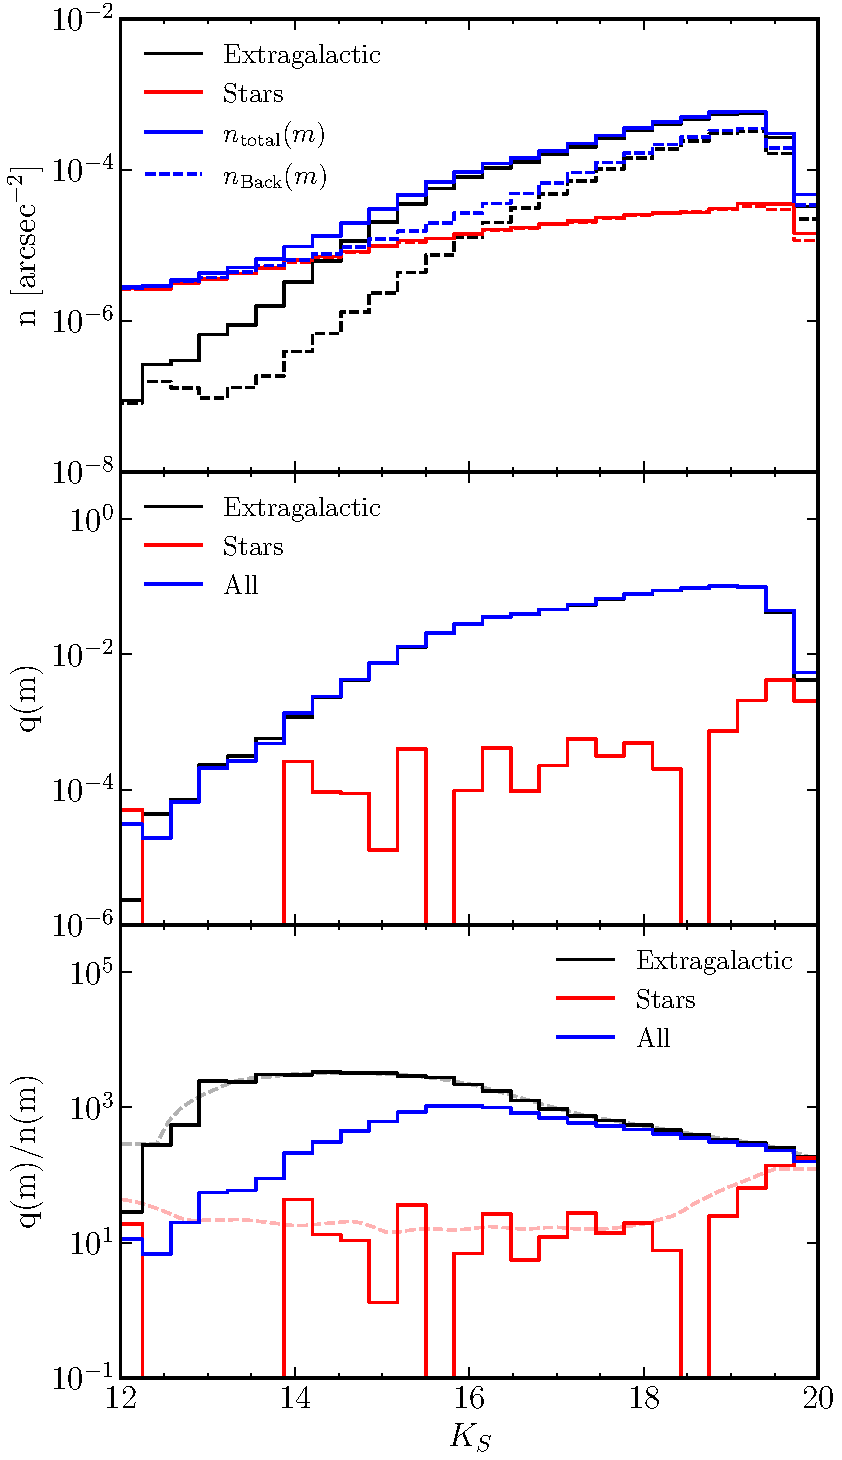
\includegraphics[height=0.75\textheight]{Figures/true_counterparts_distribution.pdf}
	\caption{Top panel: The $K_s$-band magnitude distributions of objects located within 15" of 250\,\micron \textit{Herschel} positions (blue solid line) and random positions (blue dashed line). Each histogram is also separated by extragalactic (black lines) and stellar (red lines) classification. Middle panel: The $K_s$-band magnitude distribution of "true" counterparts accounting for the excess of VIKING sources observed near \textit{Herschel} sources. Bottom panel: The ratio between the "true" counterparts distribution (middle panel) and the background distribution of sources, as used in the calculation of likelihoods - Equation \ref{eq:likelihood_ratio}. The dashed lines represent smoothed fits to $q(m)/n(m)$ to provide a continuous function at all magnitudes. The colour convention of the middle and bottom panels are the same as the top panel.}
	\label{fig:true_counterparts_distribution}
\end{figure}

\subsection{Estimating Q}

We predict the probability of finding a genuine counterpart on the VIKING images above the limiting magnitude of the near-IR survey using the method described in \citealt{Fleuren_2012}. While some methods in the literature derive $Q$ directly by totaling the $n_{\textrm{real}}(m)$ distribution and dividing by the number of SPIRE sources, this leads to a systematic overestimate due to the possibility of clustering or multiple counterparts to the same sub-mm source due to source blending. An alternative method by \citealt{Fleuren_2012} calculates an estimate of 1-$Q_0$, the probability of not observing a VIKING counterpart, by counting the number of sub-mm sources without VIKING associations within a given search radius, $r$. These sources will be given the name \textit{blanks}, and has a dependency on search radius, $B(r)$.

Blank sources may be observed in one of several scenarios. Given that the crossmatching is limited not by the \textit{Herschel} survey flux limit, but on the depth of the near-IR survey {\color{red} (Add reference to Figure if 250-flux against K-magnitude plot included)}, the most likely reason for observing a blank is that the real ID is fainter than the VIKING $K_s$-band limit. However, we may observe a blank if the counterpart lies outside the search radius or if the sub-mm source is a spurious SPIRE detection.

Even when a sub-mm source has a candidate on the VIKING images, we may not definitively say that a source is not a blank as we may encounter chance alignments with near-IR counterparts close to the same line of sight. Thus, to estimate the true number of blanks, we are reminded that the number of blanks we observe must also account for those that are spuriously identified as not blank. In other words, the number of observed blanks is the number of true blanks minus the number of true blanks that have random VIKING interlopers. If we define the number of observed blanks as $B_{\textrm{obs}}$, the number of true blanks as $B_{\textrm{t}}$ and the number of random interlopers as $N_{\textrm{rand}}$, then

\begin{equation}
    B_{\textrm{obs}} = B_{\textrm{t}} - N_{\textrm{rand}} = B_{\textrm{t}} - B_{\textrm{t}} \times f_{\textrm{rand}},
\end{equation}

where we have assumed that the number of random interlopers can be estimated from the fraction of positions that have random interlopers, $f_{\textrm{rand}}$. This fraction can be estimated from the set of random positions used above to calculate $q(m)$. Using a similar set of notation: $B_{\textrm{background}}$ to represent the number of blank positions from the catalogue of random positions; $N_{\textrm{background}}$ to represent the number of random positions and $B'_{\textrm{background}}$ representing the number of random positions for which a VIKING counterpart was observed (or "non-blank"), we can estimate $f_{\textrm{rand}}$ as:

\begin{equation}
    f_{\textrm{rand}} = \frac{B'_{\textrm{background}}}{N_{\textrm{background}}} = \frac{N_{\textrm{background}} - B_{\textrm{background}}}{N_{\textrm{background}}} = 1 - \frac{B_{\textrm{background}}}{N_{\textrm{background}}}.
\end{equation}

To scale this fraction to the size of the SGP catalogue, the same number of random positions are used as there are \textit{Herschel} positions, such that $f_{\textrm{rand}}$ may be written as:

\begin{equation}
    f_{\textrm{rand}} = 1 - \frac{B_{\textrm{background}}}{N_{\textrm{250\,\micron}}}.
\end{equation}

From substitution we observe that the fraction of \textit{Herschel} sources that are true blanks (i.e. $B_{\textrm{t}}/N_{\textrm{250\,\micron}}$), is given by

\begin{equation}
    \frac{B_{\textrm{t}}}{N_{\textrm{250\,\micron}}} = \frac{B_{\textrm{obs}}}{B_{\textrm{background}}}.
\end{equation}

In summary, to estimate 1-$Q$, we need only to divide the number of observed blank SGP positions by the number of observed blank random positions. It is clear that any estimate of $Q$ using this method depends on the given search radius from the sub-mm source, $r$, thus we calculate this fraction for a range of radii between 0" and 15" and model the dependence of $B(r) \coloneqq 1 - Q$ on the search radius in the same manner as \citealt{Fleuren_2012}. 

A sub-mm source that has no true VIKING association within a radius $r$ is either a source whose counterpart is too faint to be detected by the VIKING survey or lies outside the radius, or both. Assuming that such situations are independent of each other (i.e. a true VIKING candidate that lies at higher offsets from the sub-mm source than average is not also fainter and vice versa), then the probability of either occurring is given by the conditional probability:

\begin{equation}
\label{eq:blank_probability}
    P(\textrm{Blank}) = P(\textrm{Faint} \cup \textrm{Outside}) = P(\textrm{Faint}) + P(\textrm{Outside}) - P(\textrm{Faint} \cap \textrm{Outside}).
\end{equation}

The first term, the probability that the counterpart is too faint to be detected, is given by 1-$Q$, while the probability that the counterpart resides outside the search radius is dependent on the distribution of offsets between the counterpart and sub-mm source, $f(r)$. This distribution represents the probability that a real counterpart is found at a radial distance $r$ from the SPIRE source. We assume that the H-ATLAS sources are point-like on the 250\,\micron maps and that the errors are equal in RA and declination for radial symmetry.

While $f(r)$ naturally depends on both the positional errors of the sub-mm and the VIKING catalogues, we can assume that the near-IR positional errors are negligible compared to those of SPIRE given that the 1$\sigma$ VIKING positional errors are < 0.2" (\citealt{Fleuren_2012}). As such, we use a radially symmetric Gaussian for $f(r)$ with width $\sigma_\textrm{pos}$ corresponding to the typical SPIRE positional error. Accordingly with the theory of total probability, the probability that an observable counterpart is detected out to any search radius must equal unity, thus our function $f(r)$ is normalized such that:

\begin{equation}
    \int_0^\infty 2\pi r'f(r')dr' = 1,
\end{equation}

which implies that our function $f(r)$ take the form

\begin{equation}
    f(r) = \frac{1}{2\pi\sigma_\textrm{pos}^2}e^{\frac{-r^2}{2\sigma_\textrm{pos}^2}}.
\label{eq:positional_offset_distribution}
\end{equation}

Returning to Equation \ref{eq:blank_probability}, the probability that a VIKING counterpart is not observed within a radius $r$, P(Outside), can then be estimated from 1 - $F(r)$ where $F(r)$ relates to $f(r)$ as

\begin{equation}
    F(r) = \int_0^r 2\pi r'f(r')dr'.
\end{equation}

Upon substitution we thus find that the probability of observing a blank source as a function of the search radius can be modelled as

\begin{equation}
    B(r) = P(\textrm{Blank}) = (1-Q) + (1-F(r)) - (1-Q)(1-F(r)) = 1 - QF(r)
\label{eq:blanks_model}
\end{equation}

In Figure \ref{fig:Q_estimate} we show the observed number of blank \textit{Herschel} (open squares) and random (open circles) positions as a function of the search radius, as well as their ratio which is our proxy for $B_{\textrm{t}}/N_{\textrm{250\,\micron}}$ (filled circles). The best fitting $B(r)$ is illustrated as the black line. Using this method we measure the value of $Q$ to be $0.835\pm0.009$ when considering all VIKING objects and $Q=0.823\pm0.009$ when stellar contaminants are removed.

\begin{figure}
    \centering
	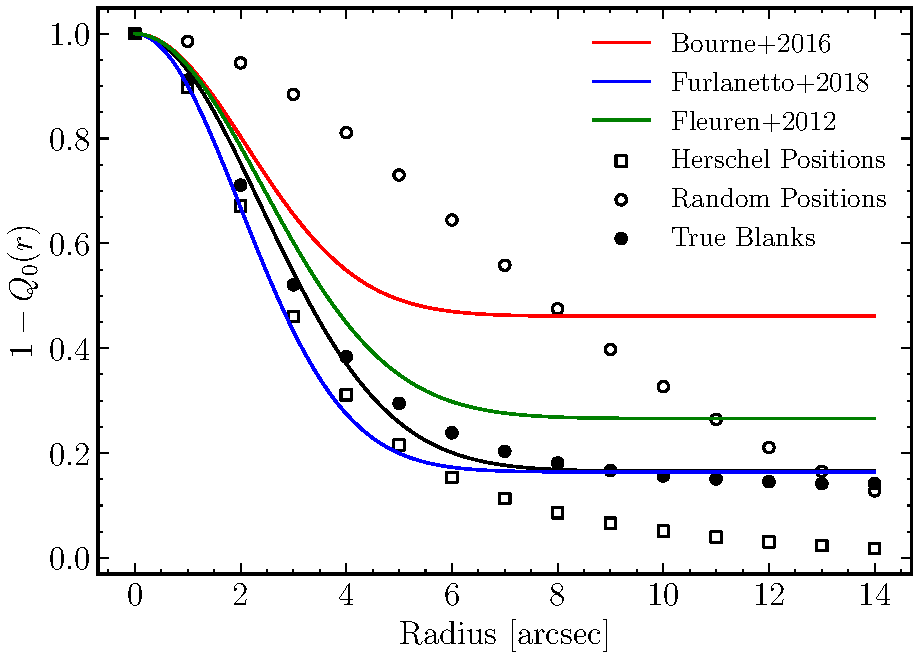
\includegraphics[width=0.75\columnwidth]{Figures/Q_estimate.pdf}
	\caption{Estimates for the number of blanks (sources without VIKING candidates) as a function of the search radius, $r$. Open circles represent the number of blank random positions placed across the SGP field, while open squares represent the number of blank SPIRE 250\,\micron positions from the H-ATLAS survey. The filled circles shows the division of the former by the latter, representing our proxy for the true fraction of SPIRE sources that are blank on the VIKING images. The solid black line represents the best fit to the points using Equation \ref{eq:blanks_model}. The same model used in \citealt{Fleuren_2012}, \citealt{Bourne_2016} and \citealt{Furlanetto_2018} are shown as green, red and blue lines respectively.}
	\label{fig:Q_estimate}
\end{figure}

Previous estimates of $Q$ from r-band SDSS candidates in the other H-ATLAS fields have taken lower values as a result of the difference in depth between SDSS and VIKING. In DR1 \citealt{Bourne_2016} measured the value of $Q$ for all SDSS objects observed in the GAMA fields to be $0.539\pm0.001$, and \citealt{Furlanetto_2018} measured a near identical value of $Q=0.538\pm0.001$ in the NGP during DR2. The value of $Q$ derived here is similar to that found by \citealt{Fleuren_2012}, $Q = 0.7342\pm0.0257$ and is almost identical to the value of $0.836\pm0.001$ found from the deep K-band analysis by \citealt{Furlanetto_2018}. As a collection, these estimates indicate that a survey of VIKING candidates returns a greater probability of observing a galaxy near a sub-mm source than an SDSS survey due to the increase in depth. This is not surprising given that the near-IR is less dust attenuated than the optical, and for higher redshifts (z > 0.5), the K-band probes the rest frame optical while the r-band selects objects at rest frame UV. This means a greater proportion of high redshift sources are included in the VIKING analysis, increasing the value of Q. A comparison between data releases and the derived Q value is made in Table \ref{tab:data_release_input_surveys} alongside their input surveys, passbands used and their limiting magnitudes.

\begin{table}
\centering
\begin{tabular}{p{3.5cm}|p{3.5cm}|p{2.5cm}|p{4cm}}
    \hline
    \hline
    H-ATLAS Release & {\color{red} Input Survey} & $Q$ Estimate & Reference \\
    \hline
    \hline
    SDP & SDSS -- ($r < 22.4$) & $0.583$ & \citealt{Smith_2011} \\ 
    Phase 1 GAMA9 & VIKING -- ($K_s < ??$) & $0.734\pm0.026$ & \citealt{Fleuren_2012} \\
    Data Release I & SDSS -- ($r < ??$) & $0.539\pm0.001$ & \citealt{Bourne_2016} \\
    Data Release II & SDSS -- ($r < ??$) & $0.538\pm0.001$ & \citealt{Furlanetto_2018} \\
    Data Release II & UKIRT -- ($K_s < ??$) & $0.836\pm0.001$ & \citealt{Furlanetto_2018} \\
    Data Release III & VIKING -- ($K_s < ??$) & $0.835\pm0.009$ & This work \\
    \hline
\end{tabular}
\caption{Comparison of the input survey passbands, depths and measured values of $Q$. From left to right the columns contain: i) the corresponding data release of H-ATLAS, ii) the input survey, passband used and limiting magnitude, iii) the fraction of true sources observed on the survey images, $Q$, iv) reference.}
\label{tab:data_release_input_surveys}
\end{table}

\subsection{Positional Uncertainty of H-ATLAS Detections}

We see in Figure \ref{fig:Q_estimate} that $B(r)$ becomes flat at approximately 3$\sigma_{\textrm{pos}}$, suggesting that few counterparts are to be found at search radii greater than $\sim$ 7". It also interesting to note that the model underpredicts the number of blank sources between 4 $\lesssim$ r $\lesssim$ 8 arcsec, but overpredicts at the highest search radii. This has been observed previously (e.g. \citealt{Fleuren_2012}) and might suggest clustering of VIKING objects which is not modelled in $B(r)$. The fitting function of Equation \ref{eq:blanks_model} also provides a prediction for the standard positional error, $\sigma_{\textrm{pos}}$, which defines the width of the positional offset distribution $f(r)$. We measure this value to be $\sigma_{\textrm{pos}} = 2.388\pm0.065$", representing the average error in the 250\,\micron positions.

The positional uncertainty has a dependency on the SNR of the sub-mm detection (\citealt{Bourne_2016}) and in theory should depend on the ratio between the FWHM of the observations and the SNR as given by

\begin{equation}
    \sigma_{\textrm{pos}} = 0.6\times\frac{\textrm{FWHM}}{\textrm{SNR}},
\label{eq:positional_uncertainty_theory}
\end{equation}

as detailed by \citealt{Ivison_2007} on the assumption of uncorrelated noise. However, the prefactor is likely to be increased by confusion noise and clustering (\citealt{Chapin_2011}; \citealt{Bourne_2014}) and so a scaling factor (typically about 1.09, corresponding to a redefined prefactor of $\sim$ 0.65) is applied and is more suitable for sources detected on sub-mm images. To define an individual value of the 1$\sigma$ positional uncertainty, and thus a separate $f(r)$ for each detection, we implement an empirical version of Equation \ref{eq:positional_uncertainty_theory} of the form

\begin{equation}
    \sigma_{\textrm{pos}} = k\times\frac{\textrm{FWHM}}{\textrm{SNR}},
\label{eq:positional_unceratinty_empirical}
\end{equation}

where $k$ is a constant to be determined. Using FWHM = 18", the fitted value of $\sigma_{\textrm{pos}} = 2.388$ and the SNR of each 250\,\micron detection, we generate a set of $k$ values and take the median value of the distribution $k = 0.66$ as the constant. This value is used in Equation \ref{eq:positional_unceratinty_empirical} to determine $f(r)$ for each object's likelihood calculation.

A more refined method of determining $\sigma_{\textrm{pos}}$ is outlined in \citealt{Smith_2011} and applied in further works (e.g. \citealt{Bourne_2014}, \citealt{Bourne_2016} and \citealt{Furlanetto_2018}), though is also an empirical measurement. In such studies, a 2D histogram is derived for the offset between sub-mm sources and optical/near-IR objects within a large box around each SPIRE source (typically 50" or more). This histogram can be modelled in shape by three contributing populations: i) a random background of chance alignments which should be observed as a constant since the probability of a chance alignment is equal along any line of sight; ii) the population of true IDs whose positional offset distribution follows $f(r)$ for a fraction $Q$ of all sources and iii) nearby counterparts that are physically correlated with the sub-mm source due to galaxy clustering but are not the true IDs, which requires an understanding of the cross-correlation between the sub-mm and optical/near-IR samples. Further details on the modelling of these histograms can be found in \citealt{Smith_2011}. By binning the sub-mm sources by their SNR and fitting the 2D histograms with a model considering the above contributions, an estimate can be made for $\sigma_{\textrm{pos}}$ as a function of SNR. Assuming a powerlaw dependence of the form $\sigma_{\textrm{pos}} = \sigma_{\textrm{pos}}(5) [\textrm{SNR}/5]^\alpha$ where $\sigma_{\textrm{pos}}(5)$ is the positional uncertainty of a 250\,\micron detection with SNR = 5, and by binning the sources again by sub-mm colour, it has been shown that the bluest SPIRE sources ($S_{250}/S_{350}$ > 2.4) have a dependence of $\sigma_{\textrm{pos}}$ on SNR that is not significantly different from the theoretical model given in Equation \ref{eq:positional_uncertainty_theory} (\citealt{Bourne_2016}; \citealt{Furlanetto_2018}). As shown in these studies the powerlaw function shifts to higher values of $\sigma_{\textrm{pos}}$ as we tend to redder sources. A possible explanation for a broader distribution of offsets for redder SPIRE sources is that an increased probability of these sources are at higher redshifts and thus there is an increased contribution from foreground structures lensing the source. To avoid this bias, $\sigma_{\textrm{pos}}$ could be measured from the 2D histogram of positional offsets of the bluest sources, but for a model dependence that is reasonable for the majority of sources, a multiplicative factor should be included, leading to the prefactor of $k$ commonly assumed being larger than 0.6. Given that the simple empirical method used here provides a similar value of $k$, we do not expect there to be any systematic differences in the likelihood calculations for SGP sources and the aforementioned papers as a result of the different methods used to calculate $\sigma_{\textrm{pos}}$.

\section{Likelihood Ratio Results}
\label{sec:lr_results}

We apply the likelihood ratio to all possible VIKING counterparts within 15" of a SPIRE source. The catalogue contains 193,527 sub-mm sources, of which 190,788 have at least one possible counterpart identified within the search radius. Having matched each source with its highest reliability counterpart we find that 181,373 (95.1\%) are sources with VIKING identifications indicating the source is a galaxy and 9,415 (4.9\%) with stellar classifications. 

In keeping with previous studies we define reliable matches as those sources with counterparts having $R \geq 0.8$ in order to minimize the number of false counterparts while maintaining a sample that is dominated by sources with a low chance of blending and thus the FIR emission is likely dominated by a single source. We identified 111,065 reliable near-IR counterparts, representing 58.2\% of all sources with at least one possible candidate. Of the reliable IDs, 110,374 (99.4\%) are classified as extragalactic and 691 (0.6\%) as stellar. The increase in the fraction of galaxies and reduction in stars compared to the input VIKING survey suggests that the LR method is highly biased against stars as is intended.

On the assumption that a source that is erroneously matched with a counterpart has a probability of $1 - R$, we can estimate the false ID rate for our reliable matches:

\begin{equation}
    N_{\textrm{False}} = \sum_{R_i \geq 0.8} (1 - R_i) = 5,343.
\label{eq:false_ids}
\end{equation}

We predict that there are 5,343 "false reliable" IDs in the SGP, representing 4.8\% of the reliable sample. This can be compared to values of 4.7\% in the GAMA fields and the NGP (optical SDSS matching), 4.5\% for the NGP (near-IR deep matching) and 4.2\% during the SDP. While the value for the SGP is in keeping with the other H-ATLAS fields, it is the highest false identification rate. It would be expected that the near-IR analyses would have the lowest false identification rates as the optical r-band restricts the limiting redshift of the counterparts to lower redshifts than the near-IR K-band. As a result, the contamination of high redshift sub-mm sources that are falsely identified with low redshift optical counterparts is expected to be higher, increasing the false identification rate. However, in the analysis of the SGP, we choose to use an increased search radius of 15" (compared to 10" as used in previous H-ATLAS studies) which increases the average number of counterparts found per source. Given the requirement of the LR method that the sum of the reliabilities of all possible candidates to a source must not exceed one, the increased average number of candidates per source reduces the average reliability of the true ID and thus increases the false identification rate - likely by a factor greater than the reduction caused by using the near-IR VIKING survey. Further discussion on the effect of increasing the search radius is made in Section \ref{sec:multiplicity}. The initial choice to use a search radius of 15" came from recent studies suggesting that genuine associations are found on the VIKING images beyond 10" as a result of gravitational lensing (\citealt{Bakx_2020}). In the final SGP \textit{Herschel}+VIKING catalogue, we wish to keep such VIKING objects despite them being highly unlikely to have significant reliability values.

The completeness, $\eta$, of the reliable sample is defined as the fraction of \textit{Herschel} sources that are recovered with a reliability greater than 0.8 (\citealt{Smith_2011}) and can be calculated as

\begin{equation}
    \eta = \frac{n(R \geq 0.8)}{n(\textrm{SNR}_{250} \geq 4) \times Q},
\label{eq:completeness}
\end{equation}

where the numerator is the size of the reliable sample and the denominator is a predictor for the true number of sources. As would be expected, a value of unity for $\eta$ would imply that the fraction of all counterparts deemed reliable has reached its theoretical maximum, $Q$. Another important diagnostic is the cleanness, $C$, of the reliable ID sample, an estimate of the number of sources that are not spurious matches, given by

\begin{equation}
    C = 1 - \frac{N_{\textrm{False}}}{N_{\textrm{250\,\micron}}}.
\label{eq:cleanness}
\end{equation}

At a reliability cut of 0.8, we find that the completeness of the extragalactic reliable sample is $\eta$ = 78\%, which is similar to the completeness values found for the NGP and GAMA fields of 74\% and 73\% respectively. Figure \ref{fig:completeness_and_cleanness} illustrates how the completeness and cleanness change over a range of different reliability thresholds. We see that a cut at $R \geq 0.8$ selects a highly clean sample at the minor expense of completeness. While an increase in the reliability cut would yield a marginally cleaner sample, it would be offset drastically by a fall in completeness. A decrease in the minimum reliability would lead to an increase in completeness at little expense of the cleanness, but to maximize the completeness would be to set a reliability so low that a one-to-one matching between sub-mm sources and counterparts would not be a guarantee. At $R \geq 0.8$ we set a boundary for which there is a good compromise between the two diagnostic parameters.

\begin{figure}
    \centering
	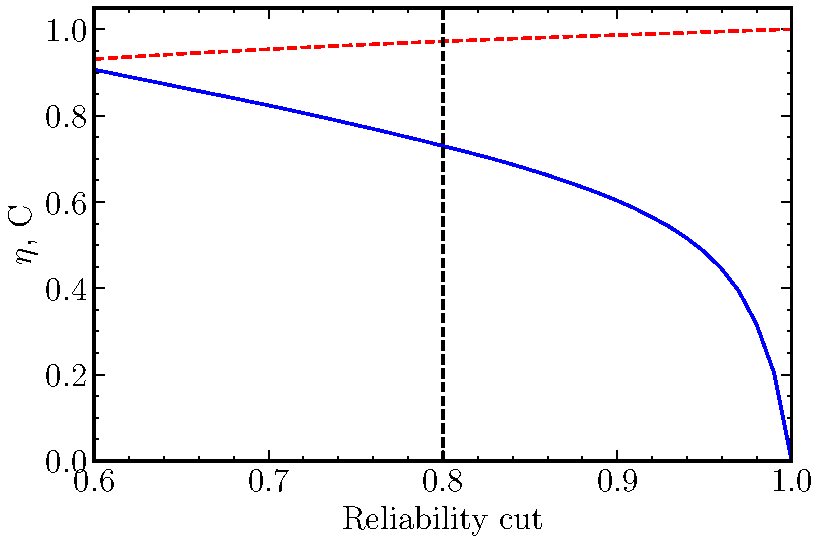
\includegraphics[width=0.75\columnwidth]{Figures/completeness_and_cleanness.pdf}
	\caption{The completeness, $\eta$, and cleanness, C, of the SGP sample as a function of various minimum cuts in reliability, illustrated as solid blue and red dashed lines respectively. The vertical dashed line reprents the minimum reliability cut used in all H-ATLAS fields (R $\geq$ 0.8).}
	\label{fig:completeness_and_cleanness}
\end{figure}

\section{Properties of \textit{Herschel} Sources and their Counterparts}

In the subsequent sections we report on the bulk properties of the SMGs in the SGP field obtained from a combination of the sub-mm and near-IR data. While the far-IR to sub-mm wavebands unveil the dusty, cold regions of the Universe, the inclusion of the near-IR data samples the peak of the emission of older stars and as such is suited for examining the stellar properties of a galaxy such as its stellar mass as it traces the total stellar content of a galaxy (\citealt{Cole_2001}; \citealt{Bell_2003}).

\subsection{Submillimeter Colours}
% Include a comparison of sub-mm colours across the data releases

\textit{
Including this section would require some additional analysis.
}

\subsection{Near-IR Properties of \textit{Herschel} Sources}
% Include a comparison of magnitude distributions

\textit{
Including this section would require some additional analysis.
}

\subsection{Multiplicity of Counterparts}
\label{sec:multiplicity}
One important disadvantage to using the LR method to identify multiwavelength counterparts to low resolution sources is that it assumes a one-to-one matching of sources and counterparts. Given that we are restricted to a user defined reliability threshold for our sample and that the sum of reliabilities for all possible candidates may not exceed one, our reliable sample becomes biased against multiple systems, such as merging galaxies, members of a cluster or non-physical associations such as confusion due to blending. The combined reliabilities of multiple systems reduces the maximum reliability of the single chosen ID. For example, consider two galaxies that form part of a cluster that are both observed on the VIKING images close to a SPIRE source. It is reasonable to imagine that these two sources may have similar K-band magnitude and radial offset from the source, and particularly if they are close to the position of the sub-mm emission, may both have high likelihoods. In such a case, either source may be considered the true ID to the source (and in reality both are likely associated), but the use of Equation \ref{eq:reliability_multiple_counterparts} to define their reliabilities leads to the following simplification (assuming the likelihoods are much larger than $1-Q$):

\begin{equation}
    R_j \sim \frac{L_j}{\sum_i L_i} \sim \frac{L_j}{2L_j} \sim 0.5.
\end{equation}

In this scenario, neither counterpart would be considered the true ID and thus we generate a bias against multiple systems. Table \ref{tab:multiplicity} shows the number of SPIRE sources and the fraction of those with reliable counterparts as a function of the number of possible candidates observed within 15". We observe that the fraction of sources with reliable counterparts decreases with increasing multiplicity. This suggests that the sample is in part incomplete because we miss sources where there are more than one genuine counterpart. In Figure \ref{fig:multiplicity} we show this reliable fraction as a function of multiplicity for the SGP compared with previous H-ATLAS studies. Comparing to the Science Demonstration Phase (\citealt{Fleuren_2012}), GAMA (\citealt{Bourne_2016}) and the NGP (\citealt{Furlanetto_2018}), we see that the SGP reliability fraction declines more slowly, peaks at slightly higher average $N_{\textrm{Match}}$ and is lower for sources where there is only a single possible counterpart. These effects are most likely a result of the increased search radius of 15" used during the SGP analysis compared to 10" in the other fields, which per source equates to a 2.5 factor increase in the search area ($A_{\textrm{SGP}}/A_{\textrm{Other}} = \pi r_{\textrm{SGP}}^2/\pi r_{\textrm{Other}}^2 = 225\pi/100\pi = 2.5$). The increased $r$ means that we are more likely to observe a reliable counterpart, but also means we increase the probability of matching erroneously to a background source, which would also explain why we observe a higher false identification rate in the SGP. The low fraction of reliably matched sources at $N_{\textrm{Match}} = 1$ may be due to an increase in unassociated VIKING objects being selected as the true ID. Occassionally, the chosen ID will be unassociated with the sub-mm source, but selected solely for being the only possible candidate despite having a large radial offset. This effect is more pronounced for an increase in $r$. In Table \ref{tab:multiplicity} we see that the average offset between the VIKING galaxy and \textit{Herschel} source is substantially higher when the galaxy is the only possible candidate, suggesting that some fraction of these sources are erroneously matched. Another reason why the reliable fraction is so low for $N_{\textrm{Match}} = 1$ is that a large fraction of the stellar candidates will fall in this bin as stars tend to be isolated (\citealt{Bourne_2016}) and therefore reduce the average reliability of these sources. On the other hand, the shift of the peak to higher $N_{\textrm{Match}}$ is likely due to the greater ability to discern between true IDs and chance alignments when the same number of candidates are spread over a larger surface area. Lastly, the increase in the search area around each SPIRE source means that the fraction of reliably matched sources does not fall until much higher $N_{\textrm{Match}}$, leading to a flatter distribution.


\begin{table}
    \centering
    \begin{tabular}{p{2cm}|p{2cm}|p{2cm}|p{2cm}|p{4cm}}
        \hline
        \hline
        $N_{\textrm{Match}}$ & $N_{\textrm{SPIRE}}$ & $N_{\textrm{Reliable}}$ & Percent & Av. Separation [arcsec] \\
        \hline
        \hline
        0 & 2,739 & 0 & 0 & 0 \\
        1 & 11,692 & 5,477 & 47 & 6.3 \\
        2 & 24,268 & 14,568 & 60 & 4.7 \\
        3 & 32,948 & 20,396 & 62 & 4.1 \\
        4 & 33,526 & 20,383 & 61 & 3.8 \\
        5 & 27,745 & 16,359 & 59 & 3.6 \\
        6 & 20,236 & 11,563 & 57 & 3.4 \\
        7 & 12,999 & 7,155 & 55 & 3.4 \\
        8 & 8,079 & 4,355 & 54 & 3.3 \\
        9 & 4,983 & 2,640 & 53 & 3.4 \\
        10 & 3,017 & 1,643 & 54 & 3.3 \\
        \hline
    \end{tabular}
    \caption{The reliable fraction illustrated as a function of the number of candidates observed per source. From left to right the columns contain: the number of possible candidates per source; the number of SPIRE sources that have the number of candidates specified in column one; the number of those sources whose best counterpart has a reliability greater than 0.8; the reliable fraction given as a percentage; and the average separation between the chosen ID and the \textit{Herschel} source in arcsec.}
    \label{tab:multiplicity}
\end{table}

\begin{figure}
    \centering
    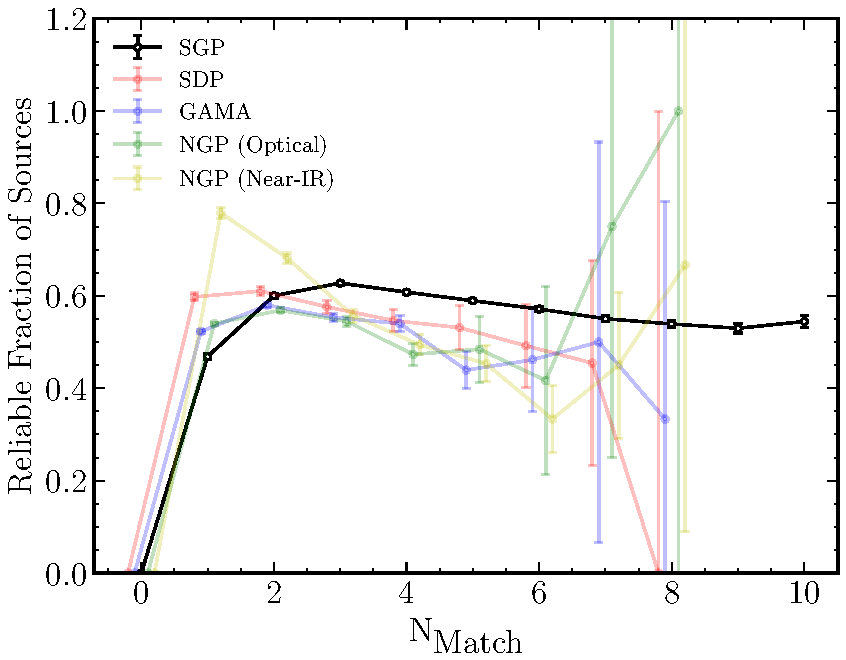
\includegraphics[width=0.75\columnwidth]{Figures/multiplicity.pdf}
    \caption{The fraction of \textit{Herschel} sources with reliably matched counterparts as a function of the number of observed candidates. The results from various H-ATLAS fields are shown as the following lines: SGP (black, this work), SDP (red, \citealt{Smith_2011}), GAMA (blue, \citealt{Bourne_2016}) and NGP (optical in green and near-IR in yellow, \citealt{Furlanetto_2018}). All other works used a maximum search radius of 10" while the SGP analysis used 15". For clarity each line has been offset in $N_{\textrm{Match}}$ by a different value.}
    \label{fig:multiplicity}
\end{figure}

We can predict the number of sources that have multiple genuine associations that were missed by the LR method by assuming that all candidates are associated with a single source if their combined reliabilities is greater than 0.8, but are missed because no individual counterpart meets the threshold. We find {\color{red} X} such sources, however, due to the increased maximum $r$ and consequently increased average number of candidates per source, even moderately valued $R$ counterparts combine to exceed the reliability cut. Alternatively, we could use the likelihood values, $L$, for each counterpart, rather than their reliability as the likelihood has no upper limit unlike the bounds on reliability, $R \in [0, 1]$. From Equation \ref{eq:reliability_multiple_counterparts} it can be seen that a reliability of 0.8 or greater corresponds to $L > 0.66$, assuming a single candidate and a value of $Q = 0.835$. An estimate for the number of lost sources with multiple associated counterparts can be made assuming that a source with a best matched counterpart with $L > 0.66$ but $R < 0.8$ is influenced by nearby candidates. We find 33,967 sources that satisfy these conditions. However, this method is also flawed as it will overestimate the true number because a large fraction of these IDs will be due to a mixture of true mergers or close groups and chance alignments. A measure for the probability that two or more counterparts are physically associated is required to potentially identify galaxy groups or mergers.

An improved estimate that removes chance alignments can be made considering the photometric redshifts of the VIKING objects (the method of obtaining photometric redshifts for the VIKING sample is presented in Section \ref{sec:phot_z_VIKING}). As shown in \citealt{Fleuren_2012}, chance matches along the line of sight can be ruled out by comparing the redshifts of all possible matches, and considering them to be associated if they fall within $\sim$ 10\% of each other for photometric redshifts or $\sim$ 5\% if using spectroscopic redshifts. While this is a simple and effective method, it does not rule out sources that happen to lie on a similar line of sight to unrelated groups or mergers of galaxies (and the true ID remaining unmatched or beyond the VIKING survey limit). In the following, we describe a new method in which we use the background distribution of VIKING sources (as used for estimating the magnitude distribution of true counterparts in Section \ref{sec:true_counterparts_distribution}) to predict the probability that a pair of VIKING galaxies with similar redshifts are associated with the sub-mm source. 

Firstly, we restrict both the SGP and background catalogues to contain only sources with two or more counterparts and restrict this further to counterparts found within 8", as this is where the majority of $L > 0.66$ counterparts are found, reducing the chance of selecting pairs of galaxies that are unrelated to the source. For each position in both catalogues, we identify the pair of galaxies with the closest redshifts and calculate the difference in their redshifts divided by the error in the difference, i.e. $\Delta z/\sigma_{\Delta z}$. In Figure \ref{fig:delta_z_multiplicity} we show the probability distribution functions (PDFs) of $\Delta z/\sigma_{\Delta z}$ for the SGP catalogue (red line) and the background catalogue (black line). When a background subtraction of the SGP catalogue is made, we observe an excess close to $\Delta z = 0$ (blue line) where the area of this peak represents the probability that a close pair of VIKING galaxies is indeed related to the SPIRE source. Fitting a Gaussian profile to the excess we calculate this probability to be 2 -- 5\% depending on the size of the bins used to generate the PDFs. By multiplying this probability by the total number of SPIRE sources for which we observe a close pair of VIKING galaxies, in this case we take this to be the width of the peak, $-0.1 \lesssim \Delta z/\sigma_{\Delta z} \lesssim 0.1$, we find an estimate for the number of \textit{Herschel} sources with genuine multiple counterparts of $\sim$ 400 -- 1,000.

\begin{figure}
    \centering
    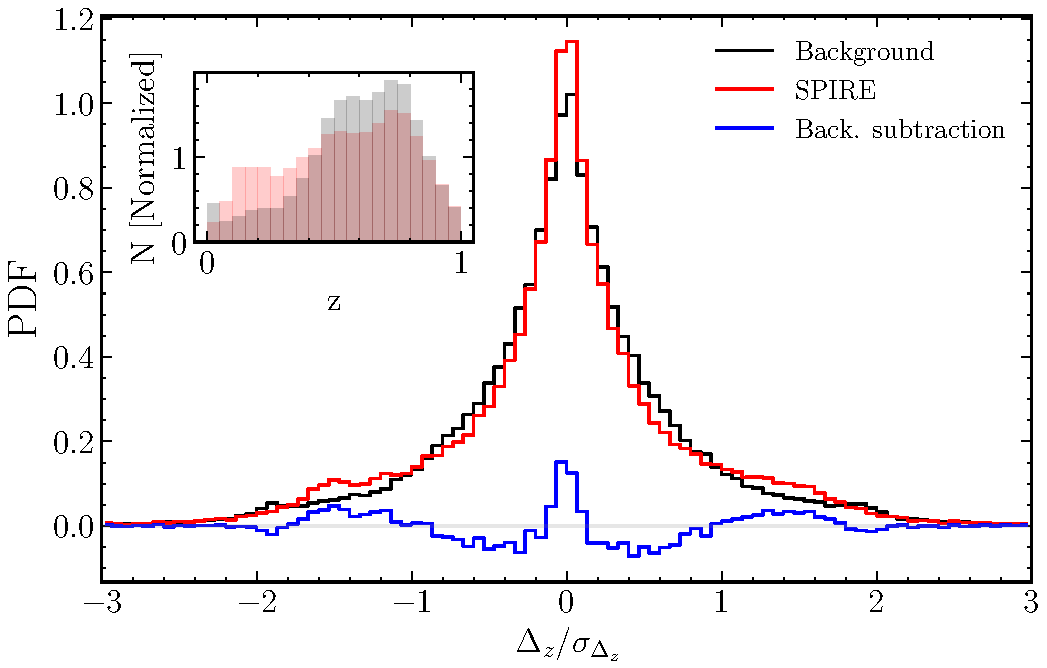
\includegraphics[width=0.75\columnwidth]{Figures/delta_z_multiplicity.pdf}
    \caption{Probability distribution functions of $\Delta z/\sigma_{\Delta z}$, the difference between photometric redshifts of VIKING counterparts divided by the error in their difference, for pairs of galaxies located within 8" of a \textit{Herschel} position in the SGP catalogue (red histogram) and randomly located positions (black histogram). The blue histogram represents a background subtraction of the former. The excess located at $\Delta z = 0$ represents the subset of VIKING galaxy pairs with similar redshifts that are associated with the SPIRE source. The inset figure shows the normalized redshift distribution of VIKING counterparts observed within 8" of the 250\,\micron positions in red and random positions in grey.}
    \label{fig:delta_z_multiplicity}
\end{figure}

It should be noted that this method is independent of the LR method, and so the pair of VIKING objects chosen for each source does not always contain the candidate with the highest reliability. In total there are 70,880 sources where we observe two or more candidates with estimated photometric redshifts (within 8" of the source), of which approximately three quarters have best counterparts that are also part of the "redshift pair". The selected pairs for the remaining quarter of sources may be the locations of unassociated galaxy interactions or multiple systems related to the sub-mm source that is overlooked by the one-to-one matching of the LR method. The subset used here is approximately one third of all sources in the SGP (70,880/193,527) and so we expect many more galaxy interactions and groups to be in the full SGP catalogue. We also note that the fraction for all sources may be higher as there is evidence to suggest that the merger rate of galaxies evolves with redshift and reaches a peak at $z \sim 1.2$ (e.g. \citealt{Bell_2006}; \citealt{Ryan_2008}). If this is true, then a large fraction of interacting systems may be beyond the VIKING detection limit and therefore lie in the blank SPIRE fields.

\subsection{Photometric Redshifts of Submillimeter Sources}
\label{sec:phot_z_Herschel}

Any study on the evolution of fundamental properties of extragalactic sources requires knowing the age of the galaxy and therefore redshift. Having crossmatched the sources detected on the sub-mm images with the sources on the VIKING images, we can begin to construct spectral energy distributions (SEDs) that places constraints on the stellar properties as well as the dust emission. The dust emission can be well approximated using a two-temperature modified blackbody model. A characteristic SED that can be used to approximate the SED of a typical H-ATLAS source is presented in \citealt{Pearson_2013} and takes the form:

\begin{equation}
    S_\nu = A[B_\nu(T_{\textrm{hot}})\nu^\beta + \alpha B_\nu(T_{\textrm{cold}})\nu^\beta],
\label{eq:pearson_sed_model}
\end{equation}

where $S_\nu$ is the flux density of the source at the rest frame frequency, $\nu$, $A$ is a normalization factor, $B(T)$ represents the Planck function at temperature $T$ (here we assume two dust temperatures, $T_{\textrm{hot}}$ and $T_{\textrm{cold}}$), $\beta$ is the dust emissivity index (the physical interpretation of this parameter is studied in depth in Chapter {\color{red} X}) and $\alpha$ represents the fraction of cold dust mass to hot dust mass. Using a sample of 40 H-ATLAS sources with spectroscopic redshifts, the optimal set of parameters were measured to be $T_{\textrm{hot}} = 46.9$\,K, $T_{\textrm{cold}} = 23.9$\,K and $\alpha = 30.1$ (assuming a fixed $\beta = 2$). This leaves a model with only two free parameters, the normalization and the redshift; a necessary simplification given that each source in the H-ATLAS SGP survey has at most three flux densities at the central wavelengths of the SPIRE bands (the PACS 100 and 160\,\micron flux densities were not included as the \textit{Herschel} images are less sensitive at these wavelengths). For each source the normalization and redshift were varied until a minimum chi squared was reached:

\begin{equation}
    \chi^2 = \sum_i \frac{(S_i - S_{i,m})^2}{E_i^2},
\end{equation}

where $S_i$ is the flux density at each SPIRE wavelength, $i$, $S_{i,m}$ is the model prediction of the flux and $E_i$ is the error on the flux. 

While all sources in the SGP have measured flux and flux errors at the SPIRE wavelengths in DR2, the errors do not account for calibration errors. The calibration error is formed of two parts: i) the main contribution comes from uncertainty in the models used for calibration objects, which in the case of SPIRE is Neptune and for PACS is a group of stars and asteroids. This error is correlated between the bands and is approximately 4\% for SPIRE; ii) a contribution uncorrelated between bands of 1.5\% (\citealt{Valiante_2016}). While the correlated error scales all fluxes by the same amount, and therefore does not impact on the $\chi^2$, the uncorrelated errors do contribute and are calculated by adding in quadrature the errors in the catalogue with the errors obtained by multiplying the flux density of each source by 1.5\% such that $E_i = \sqrt{\sigma_{S_i}^2 + (S_i \times 0.015)^2}$, where $\sigma_{S_i}$ is the error on the flux density of each source at wavelength $i$ from the H-ATLAS DR2 catalogue presented in \citealt{Valiante_2016} and \citealt{Maddox_2018}.

The upper and lower 1$\sigma$ errors on our photometric redshifts were taken at the redshifts above and below the best-fitting value at which the $\chi^2$ increases by 1. When taking all sources collectively, the mean reduced chi-squared ($\chi_\nu^2 = \chi^2/\nu$ where $\nu$ is the number of degrees of freedom) should have a value of $\sim$ 1 if the model sufficiently represents the data. A mean value of $\chi_\nu^2 > 1$ would suggest that the model is not a good representation of the data while a mean value $\chi_\nu^2 < 1$ implies that either the model has too many free parameters or that the errors on the data are too large. The $\chi^2$-minimization technique applied to the sources in the SGP yields a mean value for $\chi_\nu^2$ of 0.55. Given that the model requires only two free parameters, it is more likely that this low value is a result of overestimated flux uncertainties than the two-temperature blackbody model being an unrepresentative model for the H-ATLAS sources. While the resulting errors on the photometric redshifts account for all relevant uncertainties in the flux densities, it does not account for uncertainty in the model SED of \citealt{Pearson_2013}, given that high-redshift \textit{Herschel} galaxies have been shown to have a variety of SED shapes (\citealt{Bakx_2018}). The H-ATLAS sources used to generate the characteristic SED are intrinsically bright (facilitating their spectroscopic redshift search) and thus have fractionally smaller errors on their flux densities than the full H-ATLAS sample. This results in errors in the photometric redshifts smaller than appropriate for the variety of sources observed in H-ATLAS. For this reason, the redshift error estimated by \citealt{Pearson_2013}, $\Delta z/(1+z) = 0.12$, represents a fundamental minimum redshift error that is caused by the diversity of real galaxy SEDs and should be taken as a minimum value when applied to the SGP data. For $\sim$ 9\% of sources the measured redshift error is lower than this minimum value and we have therefore replaced the redshift error from the SED fitting with this minimum value. The median redshift of the sub-mm sources in the SGP is $\sim$ 1.4 and has a peak at a similar value. The distribution of photometric redshifts extends to very high $z$ -- we predict that more than $\sim$ 100 sub-mm sources in the SGP lie at redshifts greater than 5 -- and can be seen in Figure \ref{fig:redshift_distribution}.

\subsection{Photometric Redshifts of VIKING Counterparts}
\label{sec:phot_z_VIKING}

We obtain photometric redshifts for the VIKING counterparts by matching the catalogue to the SGP data within the \textit{Herschel} Extragalactic Legacy Project (HELP; \citealt{Vaccari_2016}; \citealt{Shirley_2019}). HELP provides an extensive catalogue of extragalactic sources observed with \textit{Herschel} over a number of fields and provides overviews of optical and near-IR surveys that are available within these regions. The method used to produce the photometric redshifts catalogued within HELP is based on the template-fitting method of \citealt{Duncan_2018a} and includes further predictions using a machine learning technique as presented in \citealt{Duncan_2018b}.

The approach combines template fitted redshifts with machine learning redshifts to create a Bayesian combination of all predicted posterior redshift distributions. Three different sets of templates were used: the default library of SEDs provided with the photometric redshift code \texttt{EAZY} (\citealt{Brammer_2008}); the XMM-COSMOS templates of \citealt{Salvato_2009} and \citealt{Salvato_2011}, which cover a wide range of galaxy spectral types as well as active galactic nuclei (AGN) and quasi-stellar object (QSO) templates; and the Atlas of galaxy SEDs presented in \citealt{Brown_2014}, a set of 129 galaxy SED templates based on a range of nearby galaxies including ellipticals, spirals and luminous IR galaxies. The machine learning algorithm uses a training set compiled from a sample of 48,995 galaxies with spectroscopic redshifts in the SGP plus additional redshifts from the three GAMA fields (the surveys used in the training set include the 2dF, 6dF, 2MRS and SRSS2 surveys). Three separate redshift estimates were made using three sets of filters: $u$, $g$, $r$ and $i$ from OmegaCAM on the VLT Survey Telescope; $g$, $r$, $i$, $z$ and $y$ from the Dark Energy Camera (DECam) on the Victor M. Blanco 4-meter Telescope; and $J$ and $K_s$ from the VISTA InfraRed CAMera (VIRCAM) on VISTA (along with the aforementioned $g$, $r$ and $i$ bands from OmegaCam). The machine learning redshifts were generated using the redshift code GPz (\citealt{Almosallam_2016}). All template and machine learning redshift posterior distributions for each source in HELP were then combined using the Hierarchical Bayesian combination method described in \citealt{Dahlen_2013}.

The method used by HELP described above provides the full photometric redshift posterior for each identified source. The assumed redshift of each object is taken from the distribution in the following way. First, an 80\% highest probability density (HPD) credible interval (CI) was calculated by starting at the peak redshift probability and lowering a threshold until 80\% of the total probability lies above the line. The resulting HPD CI may have two or more peaks, in such cases they are ranked from the most to least probable based on their peak value. We used the median redshift of the primary peak as the photometric redshift of each source. To estimate the redshift errors, we assumed that the upper and lower boundaries of the primary peak in the HPD CI defines a Gaussian, symmetric about some mean redshift value. We then transform the 80\% credible interval into 1$\sigma$ errors assuming a Gaussian distribution where an 80\% CI is equal to 1.282$\sigma$.

In total there are 29,790,690 objects with photometric redshifts in the HELP SGP catalogue. We use a 0.5" matching radius to find the nearest neighbour to all the VIKING counterparts in the H-ATLAS field. This returns 542,302 (54\%) redshifts, corresponding to 82,195 sources in the reliable ID sample (74\% of the reliable sample). Given the limiting magnitude of the VIKING survey the majority of the near-IR counterparts have redshifts < 1. This naturally represents only a fraction of all H-ATLAS sources as they extend to redshifts as high as $\sim$ 5 -- 6, but is an improvement on the depth of galaxies matched to the SDSS survey which loses its high levels of completeness beyond z $\sim$ 0.4. The distribution of redshifts for the VIKING counterparts can be seen in Figure \ref{fig:redshift_distribution}. The typical uncertainty on the redshifts is smaller for the counterparts ($\sigma_z \sim 0.21$) than it is for the sub-mm sources ($\sigma_z \sim 0.51$) as derived in the previous Section, thus to create a redshift distribution in which we have one redshift per source, we preferentially chose to use the redshift of the near-IR counterpart if avilable.

\begin{figure}
    \centering
    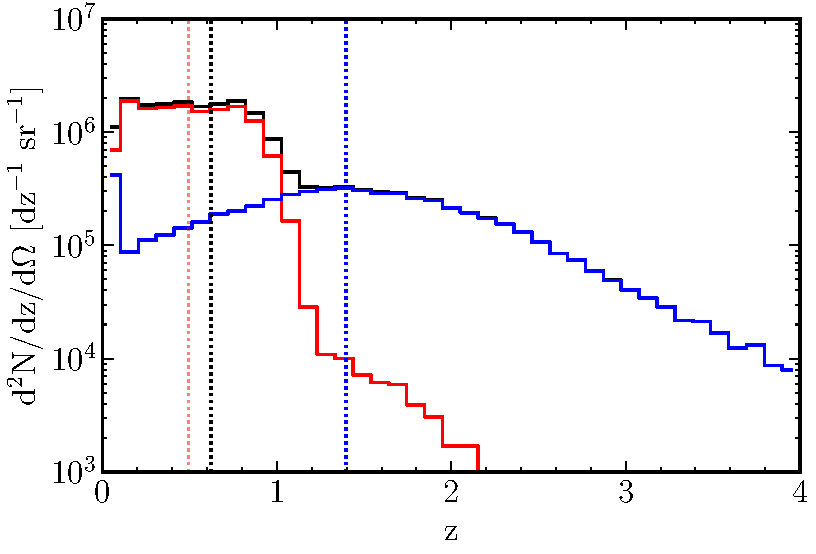
\includegraphics[width=0.75\columnwidth]{Figures/redshift_distribution.pdf}
    \caption{Photometric redshift distribution of the sources in the SGP field of H-ATLAS. The blue line represents the distribution of redshifts obtained from the SED fitting of the SPIRE fluxes to each sub-mm source; the red line represents the distribution of redshifts for the near-infrared counterparts observed in VIKING, as matched with the \textit{Herschel} Extragalactic Legacy Project, and the black line represents the distribution of the best estimate for each source, preferentially selecting the redshift of the counterpart. The median redshifts are $z_{\textrm{sub-mm}} = 1.40$, $z_{\textrm{near-IR}} = 0.49$ and $z_{\textrm{best}} = 0.62$ and are illustrated by the dotted red, blue and black vertical lines respectively.}
    \label{fig:redshift_distribution}
\end{figure}

\section{Gravitational Lensing in the SGP}

When the light from a distant galaxy is close to the same line of sight as a foreground mass, whether that be an individual galaxy (likely a massive elliptical) or galaxy cluster, the magnification of the background source due to the deflection of the light makes the galaxy appear brighter with a larger angular size. This gravitational lensing effect makes these systems ideal targets for studying intrinsically faint and distant galaxies that may otherwise be impossible to probe. This effect can be exploited to generate prime targets for studies of the physical conditions in distant star forming galaxies at resolutions otherwise unattainable and also provide potential as subjects for studies of the cosmological parameters (e.g. \citealt{Kochanek_1992}; \citealt{Kochanek_1996}; \citealt{Grillo_2008}; \citealt{Oguri_2012}; \citealt{Eales_2015}) and the evolution of the equation of state of dark matter (e.g. \citealt{Zhang_2009}). 

However, identifying large samples of lenses can be time-consuming when searches for lensed sources are made from large surveys with observationally expensive follow up imaging to find the signs of gravitational lensing (e.g. Einstein rings). Moreover, if a blind search for lensing events were made it would require large areas to be surveyed due to their rarity. However, blank field sub-mm surveys have been shown to contain a vast number of lensing events, easily identifiable as the brightest sources on sub-mm images (e.g. \citealt{Blain_1996}; \citealt{Perrotta_2002}; \citealt{Negrello_2007}; \citealt{Paciga_2009}; \citealt{Bakx_2020}). We note that the occurence of gravitational lensing events can be high in the sub-mm because of the high average redshift (z $\gtrsim$ 1) of sub-mm selected galaxies. The brightest sources (typically selected using a flux cut of $S_{\textrm{500\,\micron}} \gtrsim$ 100\,mJy) that populate the bright tail of the sub-mm counts contain several populations. These include low redshift (z $\lesssim$ 0.1) spiral and starburst galaxies, higher redshift AGNs and lensed sources. Given that the former populations can be easily identified and removed from shallow optical and radio surveys, a flux-limited sample of sub-mm sources can provide a sample of candidate lensing systems with low contamination. This method has been used extensively in previous studies of \textit{Herschel} surveys. \citealt{Negrello_2010} produced the first sample of strongly lensed \textit{Herschel} galaxies (SLGs) presenting 5 lensed galaxies within the SDP. This was followed by the study of \citealt{Wardlow_2013} that identified 11 lensed galaxies from the 95\,deg$^{2}$ area of the \textit{Herschel} Multi-tiered Extragalactic Survey (HerMES; \citealt{Oliver_2012}). \citealt{Nayyeri_2016} presented a further 77 candidates from the 372\,deg$^{2}$ of sky covered by the HerMES Large Mode Survey (HeLMS) and the \textit{Herschel} Stripe 82 Survey (HerS; \citealt{Viero_2014}). More recently, \citealt{Negrello_2017} identified a sample of 80 candidates for lensing from $\sim$ 600\,deg$^{2}$ of the H-ATLAS. In the subsequent sections we shall present a statistical sample of candidate lensed sources from the SGP, first by selecting the brightest sources using the method outlined in \citealt{Negrello_2017}, then extending this to lower flux densities by predicting the likelihood of gravitational lensing based on the redshift distributions of the sub-mm sources and their near-IR counterparts. 

\subsection{The Brightest Lensed Sources}
\label{sec:brightest_lenses}

The number counts of unlensed sources falls rapidly at 500\,\micron flux densities above $\sim$ 100\,mJy because of the steep luminosity function of SMGs. For a given luminosity, the probability of a galaxy having an intrinsic brightness of such high flux density becomes much lower than the probability that an intrinsically fainter source is magnified due to gravitational lensing. Selecting all sources in the SGP with $S_{\textrm{500\,\micron}}$ > 100\,mJy we obtain 179 sources, 175 of which had at least one associated VIKING counterpart. 

The low-redshift spirals and flat spectrum radio galaxies that contaminate this sample were identified and removed by searching the location of the sources with the NASA/IPAC Extragalactic Database (NED). We also removed two variable stars (HATLASJ012658.0-323234 -- R Sculptoris and HATLASJ225519.6-293644 -- V Piscis Austrini) and five blazars, as listed in Table \ref{tab:blazars}. In total 131 local galaxies were clearly identified from their resolved imaging in NED. These objects have much "bluer" sub-mm colours than the remaining sample, suggesting that despite their equally high flux density they are separate populations at different redshifts. The remaining 41 sources with "redder" sub-mm colours and thus most likely to be at high redshifts, were retained as our list of bright candidate lensed sources in the SGP. The complete sample of sources is tabulated in Appendix \ref{app:candidate_lenses_bright}. Figure \ref{fig:submm_colours_lensed_candidates} shows a plot of $S_{\textrm{250\,\micron}}/S_{\textrm{350\,\micron}}$ against $S_{\textrm{350\,\micron}}/S_{\textrm{500\,\micron}}$ for all 179 sources with $S_{\textrm{500\,\micron}}$ > 100\,mJy, coloured according to their classification (local galaxies in black, variable stars in blue, blazars in green and all remaining sources in red). As illustrated in \citealt{Negrello_2017} the bimodality of the colour-colour plane reflects the two sets of populations being at very different redshifts. The suggestion from this plot is that a relatively clean sample of lensed candidates (barring possible blazars) can be obtained solely from submillimeter fluxes alone.

\begin{table}
    \centering
    \begin{tabular}{p{4.5cm}|p{3cm}|p{1.75cm}|p{1.75cm}|p{1.75cm}}
        \hline
        \hline
        H-ATLAS IAU Name & NED Identification & $S_{\textrm{250\,\micron}}$ [mJy] & $S_{\textrm{350\,\micron}}$ [mJy] & $S_{\textrm{500\,\micron}}$ [mJy] \\
        \hline
        \hline
        HATLASJ014310.0-320056 & PKS 0140-322 & 96.0$\pm$7.5 & 119.5$\pm$8.4 & 122.4$\pm$9.0 \\
        HATLASJ014503.4-273333 & [HB89] 0142-278 & 131.4$\pm$7.8 & 179.2$\pm$8.8 & 234.4$\pm$9.0 \\
        HATLASJ222321.6-313701 & PKS 2220-318 & 86.0$\pm$9.5 & 110.9$\pm$10.5 & 131.9$\pm$11.7 \\
        HATLASJ224838.6-323551 & [HB89] 2245-328 & 119.2$\pm$7.7 & 152.8$\pm$8.3 & 194.7$\pm$8.6 \\
        HATLASJ235347.4-303746 & PKS 2351-309 & 77.1$\pm$7.4 & 96.6$\pm$8.4 & 103.1$\pm$8.9 \\
        \hline
    \end{tabular}
    \caption{The blazars with 500\,\micron flux density > 100\,mJy identified in the SGP using NED.}
    \label{tab:blazars}
\end{table}

The 41 bright candidates include 30 that were previously identified in \citealt{Negrello_2017}. The 11 additional sources fall outside of the mask of the SGP used in this study, which was initially used to remove the edges of the survey area which had fewer scans from the \textit{Herschel}-SPIRE instrument and thus were affected by higher noise. While the method described here only goes as far as to suggest that these \textit{Herschel} sources are at high redshift (the chance of them actually being lensed is purely dependent on the ratio between the probability that a source with a given 500\,\micron flux is lensed and the probability it is not), at the time of publication of \citealt{Negrello_2017}, optical (SDSS or KiDS) to near-IR (UKIDSS-LAS, VIKING or HST/F110W) imaging had only discounted one source from the initial sample for not being strongly lensed, and 28 sources fall into the broad categories of confirmed strong lensing or likely lensed sources. Follow up imaging of these sources appear to confirm the idea that the brightest \textit{Herschel} sources are dominated by gravitational lensing events. Previous studies predict that the surface density of SLGs above 100\,mJy at 500\,\micron is $\sim$ 0.1 -- 0.2\,deg$^{-2}$ (\citealt{Vieira_2010}; \citealt{Wardlow_2013}; \citealt{Nayyeri_2016}). Assuming that all 41 sources in the SGP are being lensed, the surface density of lensed sources is 0.14\,deg$^{-2}$. It is interesting to note that two sources with $S_{\textrm{500\,\micron}}$ > 100\,mJy have no VIKING counterpart within 15" and a further 13 do not have photometric redshifts from HELP. These bright systems may be interesting examples of sources where the lens is at a high redshift (beyond z $\sim$ 1), sources that are lensed by a cluster, or not be lensed at all.

\begin{figure}
    \centering
    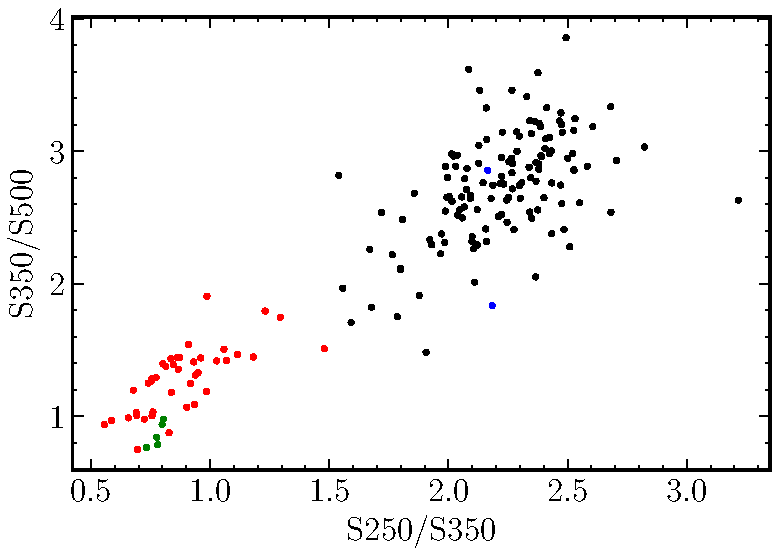
\includegraphics[width=0.75\columnwidth]{Figures/submm_colours_lensed_candidates.pdf}
    \caption{A colour-colour diagram ($S_{\textrm{250\,\micron}}/S_{\textrm{350\,\micron}}$ against $S_{\textrm{350\,\micron}}/S_{\textrm{500\,\micron}}$) for objects with $S_{\textrm{500\,\micron}}$ > 100\,mJy in the SGP. Sources are coloured according to their classification: local galaxies (black), variable stars (blue), blazars (green) and the remaining sources that we take as our candidates for lensing events (red).}
    \label{fig:submm_colours_lensed_candidates}
\end{figure}

\subsection{Extending the Search for Lenses to Lower Fluxes}

While selecting the brightest sub-mm sources is an easy and effective method for sampling those with the highest probability of lensing, the chance of a \textit{Herschel} source being lensed need not be dependent on its intrinsic brightness and many lensing events are missed because their magnification factors do not substantially lift their fluxes above the level of other, more intrinsically bright unlensed sources.

An alternative way to predict the probability that a source is lensed is to compare the redshifts of the near-IR counterparts and the sub-mm source, assuming that the counterpart is a foreground deflector and not the true galaxy producing the dust emission. If the redshift of the foreground counterpart is much lower than the the redshift for the dust emission, it suggests that the two sources are unrelated and raises the probability that the \textit{Herschel} source is lensed.

Comparing the distribution of properties of sub-mm sources and their counterparts has already been used in previous studies to predict gravitational lensing events; a notable example of this being the Statistical \textit{Herschel}-ATLAS Lensed Objects Selection (SHALOS; \citealt{Gonzalez-Nuevo_2019}) which was used to predict that there are several hundred SLG candidates in the GAMA and NGP fields. The SHALOS analysis assigns a probability of gravitational lensing for each source in a catalogue based on the similarity between the properties of the sub-mm source and the properties of the cross-matched optical counterpart. In \citealt{Gonzalez-Nuevo_2019} these properties include the redshift distributions (the greater their disparity the higher the probability); the angular separation of the source and object (the closer to the same line of sight the higher the probability); the ratio between the optical and sub-mm flux densities; and the luminosity of the source (though this final property does not rely on a comparison between the source and counterpart, but rather a comparison to the luminosities of other galaxies at similar redshifts). For simplicity we chose to implement a similar metric for the sources in the SGP but only using the photometric redshift distributions. The reason for this is two-fold. First, the flux density ratio and luminosity parameters require a comparison with other galaxies. To derive a probability from the luminosity of a galaxy, the galaxy in question needs to be compared with similar galaxies at the same redshift and to estimate a probability from the flux density ratios requires a knowledge of a typical \textit{Herschel} SED at a given redshift. Both of these comparisons mean that the method is not self-contained and thus not a method that can be applied to a set of sources with no prior knowledge. Secondly, the angular separation of the source and counterpart in this analysis suggests that the closer the two signals are to the same line of sight, the higher the probability that they are lensed. While this is true of galaxy-galaxy strong lensing events, the distribution of angular offsets between sub-mm sources and optical/near-IR counterparts suggests that lensing by galaxy groups and clusters may contribute more significantly to the number of lensing events at fainter flux densities than galaxy-galaxy lensing events (\citealt{Bakx_2020}). The above method would have an intrinsic bias against lensing events involving foreground groups and clusters.

The Bhattacharyya coefficient gives an approximation of the overlap between two distributions and is used to compare the redshift distributions of all sources in the SGP. Assuming two continuous redshift probability distributions $p_1$ and $p_2$, the Bhattacharyya coefficient is defined as

\begin{equation}
    BC(p_1, p_2) = \int \sqrt{p_1(z) p_2(z)} dz.
\end{equation}

The Bhattacharyya coefficient is closely related to the Bhattacharyya distance, $D(p_1,p_2)$, which is defined as

\begin{equation}
    D(p_1, p_2) = -\textrm{ln}[BC(p_1, p_2)].
\label{eq:Bhattacharyya_distance}
\end{equation}

Assuming that our probability distributions are well approximated by a Gaussian with means $\mu_1$ and $\mu_2$ and standard deviations $\sigma_1$ and $\sigma_2$, the Bhattacharyya distance can be simplified to

\begin{equation}
    D(p_1, p_2) = \frac{1}{4}\textrm{ln}\Bigg[\frac{1}{4}\Bigg(\frac{\sigma_1^2}{\sigma_2^2}+\frac{\sigma_2^2}{\sigma_1^2}+2\Bigg)\Bigg] + \frac{1}{4}\Bigg[\frac{(\mu_1 - \mu_2)^2}{\sigma_1^2 + \sigma_2^2}\Bigg].
\label{eq:Bhattacharyya_distance_gaussian}
\end{equation}

The final step in calculating the lensing probability of each source, $p_{\textrm{lens}}$, is to let $p_{\textrm{lens}} = 1 - BC(p_1, p_2)$, as it is through a disparity in the two redshift values that we expect to observe candidates for lensing. For the VIKING galaxy to be the lens magnifying the sub-mm emission, the source must be at a much higher redshift than the near-IR counterpart. To ensure we are not biased by systems where the median redshift of the counterpart is higher than the source due to catastrophic photometric redshift errors, we add to the lensing probability any area of the normalized probability distribution of the sub-mm source that lies below $\mu_\textrm{near-IR} - 3\sigma_\textrm{near-IR}$. Given that most sources have large errors on the near-IR redshift ($\sim$ 50\%), this additional term is negligible for most sources, but suppresses the probability for those sources where $z_\textrm{near-IR} > z_\textrm{sub-mm}$. When this abbreviated version of the SHALOS method is applied to the SGP we find that no source with $p_{\textrm{lens}} \gtrsim 0.6$ is affected by such contaminants. Figure \ref{fig:lens_probability_scatter} shows a comparison of the near-IR redshifts and sub-mm redshifts of all sources in the SGP, coloured by their respective lensing probability using Equations \ref{eq:Bhattacharyya_distance} and \ref{eq:Bhattacharyya_distance_gaussian}. The limiting $K_s$-band magnitude of the VIKING survey prohibits a high completeness fraction of matches above $z_\textrm{near-IR} \sim 1$. Due to the larger average error on the \textit{Herschel}-SPIRE redshifts, a high percentage of sources lie at positions where $z_\textrm{sub-mm}$ is much greater than $z_\textrm{near-IR}$. To ensure we do not include a substantial number of false candidates in our lensed catalogue, we must only take as potential lensing candidates those sources whose redshifts are so discrepant they are not statistically significant with the 1:1 line within the large photometric errors.

\begin{figure}
    \centering
    \includegraphics[width=0.75\columnwidth]{Figures/lens_probability_scatter.pdf}
    \caption{Scatter plot showing a comparison between the redshifts measured from the sub-mm flux densities of each source with the redshift obtained from the \textit{Herschel} Extragalactic Legacy Project matched to the VIKING near-IR counterparts. Each source is coloured by the probability that it represents a lensing system according to Equations \ref{eq:Bhattacharyya_distance} and \ref{eq:Bhattacharyya_distance_gaussian}. The 1:1 line is illustrated as a dashed black line and the average uncertainty in both redshift estimates for an individual source is shown.}
    \label{fig:lens_probability_scatter}
\end{figure}

Having derived a value of $p_{\textrm{lens}}$ for each \textit{Herschel} source, we require a threshold value above which would suggest it should be included in our lensed catalogue. The rationale for this value is that $p_{\textrm{lens, thr}}$ should construct a sample of candidates with the fewest contaminating unlensed sources (potentially at the expense of having a smaller catalogue). This requires a knowledge of the probability that a given source is not lensed, and while it is not possible without time consuming follow up imaging to determine if a source shows signs of gravitational lensing, we can estimate this probability statistically for the whole sample. This allows us to predict the number of contamination unlensed sources we might expect in our catalogue and select the value of $p_{\textrm{lens}}$ that minimizes this false positive rate. We estimated the false positive rate in two ways. First, the probability of any source, $i$, not being lensed is given by $1 - p_{\textrm{lens, i}}$, thus the sum

\begin{equation}
N_{\textrm{not lensed, 1}} = \sum_{i}^{N_{\textrm{lenses}}}{1 - p_{\textrm{lens, i}}}
\label{eq:unlensed_estimate_1}
\end{equation} 

of all sources above some value of $p_{\textrm{lens}}$ predicts the number of spuriously selected unlensed sources that would contaminate the resulting sample. 

The second estimate comes from the fact that the Likelihood Ratio analysis leads to a false identifiation rate, where the sub-mm source is expected to be matched to the wrong counterpart in a certain fraction of instances. We showed earlier that the LR method applied to the H-ATLAS SGP field would have erroneously matched VIKING counterparts for 4.8\% of sources (Section \ref{sec:lr_results}). This means that for 4.8\% of all sources with a counterpart matched at greater than 80\% probability, there is likely no association between the source and the near-IR counterpart. The second prediction of the number of unlensed contaminants therefore comes from the the fraction of our spuriously matched sources that would end up in our lensed catalogue at a given threshold probability. We predicted this number of sources by taking the number of counterparts in the reliable sample, multiplying by the false identification rate, and then multiplying again by the fraction of sources that are at a high enough redshift that the difference between the the sub-mm redshift and the redshift of the counterpart is large enough for the source to be more likely classified in the lensed catalogue than not. Assuming a VIKING counterpart with $z_\textrm{near-IR} \sim 0.5$, the lower limit for $z_\textrm{sub-mm}$ is predicted to be $\sim$ 2.5. This estimate can thus be written as follows:

\begin{equation}
N_{\textrm{not lensed, 2}} = N_{\textrm{Reliable}} \times f_{\textrm{False}} \times f_{\textrm{(z > 2.5)}}.
\end{equation} 

The two methods, $N_{\textrm{not lensed, 1}}$ and $N_{\textrm{not lensed, 2}}$ are combined and divided by the total size of the lensed catalogue to define the probability of observing a false positive (any given source in our lensed catalogue not being part of a lensed system) as a function of $p_{\textrm{lens}}$, which is illustrated in Figure \ref{fig:lens_false_positive}.

\begin{figure}
    \centering
    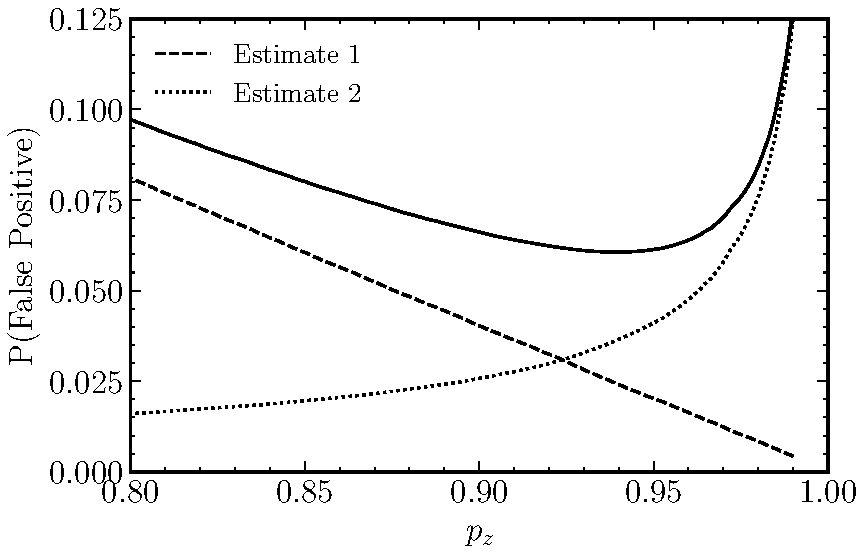
\includegraphics[width=0.75\columnwidth]{Figures/lens_false_positive.pdf}
    \caption{The false positive rate (the fraction of sources in the lensed catalogue that are expected to not be part of a lensing system) as a function of the threshold probability for gravitational lensing, $p_\textrm{lens}$, as calculated using Equations \ref{eq:Bhattacharyya_distance} and \ref{eq:Bhattacharyya_distance_gaussian}. The false positive rate is split into two components: the first calculated assuming that the probability of any source, $i$, not being lensed is given by $1 - p_{\textrm{lens, i}}$ (dashed line), the second estimated from the fraction of sources in the reliable (R > 0.8) SGP sample that are likely to be spuriously matched to a VIKING counterpart and have a sub-mm predicted redshift large enough that the source is more likely contained in the lensed catalogue than not (dotted line). The total is the combination of the two estimates (solid line). The optimal probability threshold defining our lensed catalogue is found at the minimum false positive rate. This occurs at $p_\textrm{lens, thr} = p_\textrm{lens} = 0.94$ and represents a false probability rate of $\sim$ 6\%. {\color{red} (Change axis to $p_\textrm{lens}$).}}
    \label{fig:lens_false_positive}
\end{figure}

A notable disadvantage of this method, however, is that it relies on the requirement that a counterpart is identified on the VIKING image at the location of the \textit{Herschel} source and that it is matched with a high probability. In reality, these reliable matches are expected to be the locations where we are most confident that the VIKING object that we observe is the cause for the dust emission, and likely represents a smaller fraction of lensing events than all other "unreliable" sources. This leads to our prediction being an underestimate of the true number of lensing events. In this case it is a necessary requirement to calculate $N_{\textrm{not lensed, 2}}$ as the false identification rate is highly uncertain for lower reliability thresholds.

In Figure \ref{fig:lens_false_positive} we see that $N_{\textrm{not lensed, 1}}/N_{\textrm{lensed}}$ decreases steadily for increasing $p_{\textrm{lens}}$. This is as expected given the decrease in the size of the lensed catalogue with $p_{\textrm{lens}}$. $N_{\textrm{not lensed, 2}}/N_{\textrm{lensed}}$, however, increases steadily until a rapid rise beyond $p_\textrm{lens} \sim 0.95$. {\color{red} Reasoning.} The combination of the two methods gives a function with a minimum value at $p_\textrm{lens} = 0.94$, which we took to be the optimal probability threshold for gravitational lensing. Assuming this value we predict that the resulting sample of candidate lenses in the SGP has a contamination rate of $\sim$ 6\%. Using the following criteria: i) the \textit{Herschel} source must have an observed VIKING counterpart with a crossmatching reliability of > 0.8 from the LR method and a corresponding redshift; ii) the 500\,\micron flux density must not exceed 100\,mJy (so as to not influence the method used in Section \ref{sec:brightest_lenses}) and iii) the probability of lensing calculated from the Bhattacharyya coefficient is greater than 0.94, we identified 5,923 candidates for gravitational lensing within the SGP field below 100\,mJy at 500\,\micron.

We applied the method described in this section to the subset of sources with $S_{\textrm{500\,\micron}}$ > 100\,mJy for which we can estimate $p_\textrm{lens}$. From the 41 candidates listed in Appendix \ref{app:candidate_lenses_bright}, 24 have near-IR counterparts with R > 0.8 and 19 of these have a photometric redshift from the HELP catalogue. In most cases the probability of gravitational lensing is greater than 0.95 and the mean probability is 0.89. This provides additional evidence to suggest that the brightest sources are indeed being lensed by VIKING foreground deflectors.

\subsection{Number Counts and Redshift Distribution of Lensed Candidates}

To assess how well this simple method for selecting lensing events in the H-ATLAS compares to galaxy evolution models, we compared the redshift distribution, number counts and the fraction of all sources that are candidate lenses with the predictions made by the evolution model of \citealt{Cai_2013}, as illustrated in Figure \ref{fig:lens_distributions_against_cai}. When comparing the source counts from the $\sim$ 16\,deg$^{2}$ SDP field to a selection of models, it was found that the model of \citealt{Negrello_2007} gave the closest match to observations (\citealt{Clements_2010}). Given that the work of \citealt{Cai_2013} is a development of the \citealt{Negrello_2007} model and it also incorporates the effect of strong gravitational lensing, it should be suitable for comparison with the observations in the SGP. The model of \citealt{Cai_2013} combines a physical, forward model for protospheroidal galaxies and AGN at z $\geq$ 1.5 with a phenomenological backward model for late-type galaxies. The protospheroidal galaxies were modelled on the work of \citealt{Granato_2004} where these sources are viewed as massive protospheroids that are in the process of forming their stellar mass. At lower redshifts, the model assumes a combination of 'warm' starburst galaxies and 'cold' normal-type galaxies. The model incorporates the effect of gravitational lensing on the observed source counts of these galaxies at IR wavelengths, assuming a fixed magnification value. To compare with the lensed candidates described here, we chose to use a variant of the \citealt{Cai_2013} model where the maximum magnification due to gravitational lensing is $\mu$ = 12, a value that provides good agreement with the lensed number counts of \citealt{Negrello_2017}.

We combined all sources that have $p_{\textrm{lens}} > 0.94$ with the bright $S_{\textrm{500\,\micron}}$ > 100\,mJy candidates to form a complete sample across the SGP. In the top panel of Figure \ref{fig:lens_distributions_against_cai} we show the redshift distribution for all sources (solid black line) and the distributions of $z_{\textrm{sub-mm}}$ and $z_{\textrm{near-IR}}$ for the lensed sample (red and pink solid lines respectively). The predictions from the \citealt{Cai_2013} model are shown as dashed lines using the same colour convention. The distributions show that while the total number of sources is well predicted by the model, there is a large discrpenancy in the number of lensed systems at all redshifts above z $\sim$ 0.5. When illustrated as a function of the 500\,\micron flux density (middle panel), we now see that the \citealt{Cai_2013} model matches the predictions for the SGP well at flux densities above $\sim$ 60\,mJy but there is a large disagreement at the lowest flux densities towards the 4$\sigma$ detection limit. Note that while the SGP lensed counts fall below the model and the samples of \citealt{Negrello_2017} and \citealt{Nayyeri_2016} at flux densities greater than $\sim$ 150\,mJy, it had already been shown by \citealt{Negrello_2017} that there is a considerable underdensity of lensed galaxies at the highest fluxes compared to other H-ATLAS fields and thus this drop is not unexpected. This discrepancy is corroborated by the lensing fraction -- the fraction of all galaxies that are likely being lensed -- shown in the bottom panel of Figure \ref{fig:lens_distributions_against_cai}. While the model predicts that the probability of lensing is very low and approaching zero at low flux densities, the candidate lenses in the SGP continue to contribute $\sim$ 10\% to the total source counts at the detection limit of the survey at 500\,\micron.

A likely explanation for the underprediction of the \citealt{Cai_2013} model is that it is limited to strong lensing ($\mu$ > 2) events, whereas our simple method relies solely on the redshifts of the galaxies and thus is not limited by their apparent brightness. Studies of the spatial cross-correlation between sub-mm galaxies in the GAMA fields and SDSS galaxies (\citealt{Gonzalez-Nuevo_2014}; \citealt{Gonzalez-Nuevo_2017}) have shown that the amplification of clustered sub-mm galaxies by foreground structures can be explained by weak gravitational lensing ($\mu$ < 2). Although the cross-correlation signal cannot be reconstructed solely from galaxy-galaxy weak lensing, it can be reproduced on sub-arcminute scales if the foreground objects act as markers for galaxy groups or clusters. On larger scales the cross-correlation is believed to reflect the clustering of the haloes from these galaxy groups and clusters. We may therefore ask ourselves whether VIKING galaxies act as signposts to the locations of galaxy groups or clusters and thus our inflated prediction for the number of lensed candidates is in part the result of observing a collection of strong and weak lensing events. As noted in \citealt{Gonzalez-Nuevo_2017}, strong lensing becomes a non-negligible contribution to the cross-correlation signal below $\sim$ 30" and increases to smaller radii. This means that despite galaxy groups and clusters being the dominant contribution to the cross-correlation, the effects of gravitational magnification on the number counts of \textit{Herschel} sources are dominated by galaxy-galaxy strong lensing. From this we might expect that the brightest sources are those where the VIKING counterpart is closest to the same line-of-sight as the \textit{Herschel} source, generating the largest magnification factors (and thus matching the predictions from \citealt{Cai_2013} assuming $\mu$ > 2), while the fainter lensed galaxies represent small magnifications of the sub-mm source due to weak lensing from potential galaxy clusters and groups.

\begin{figure}
    \centering
    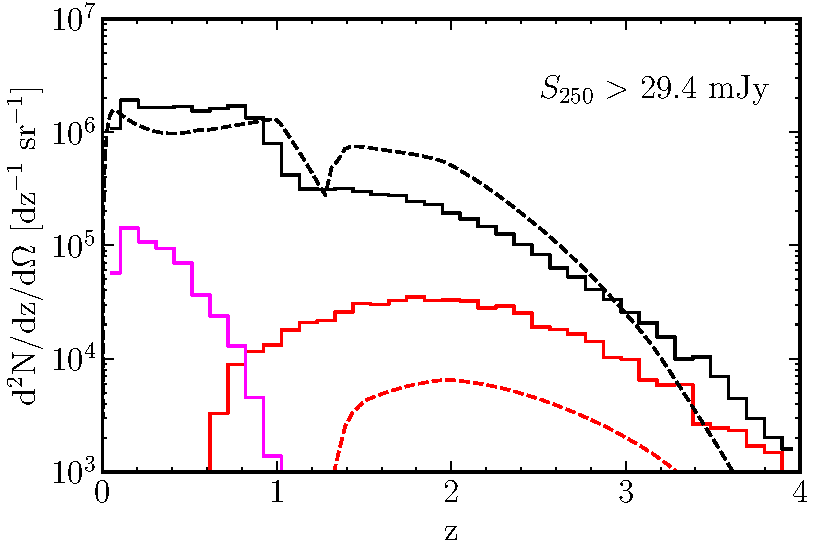
\includegraphics[width=0.5\columnwidth,height=0.24\textheight]{Figures/lens_redshift_distribution.pdf}
    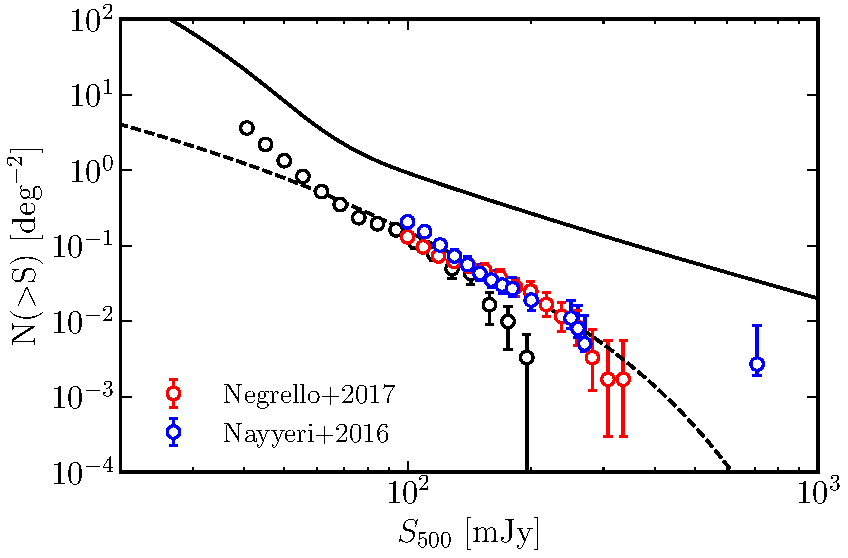
\includegraphics[width=0.5\columnwidth,height=0.24\textheight]{Figures/lens_number_counts.pdf}
    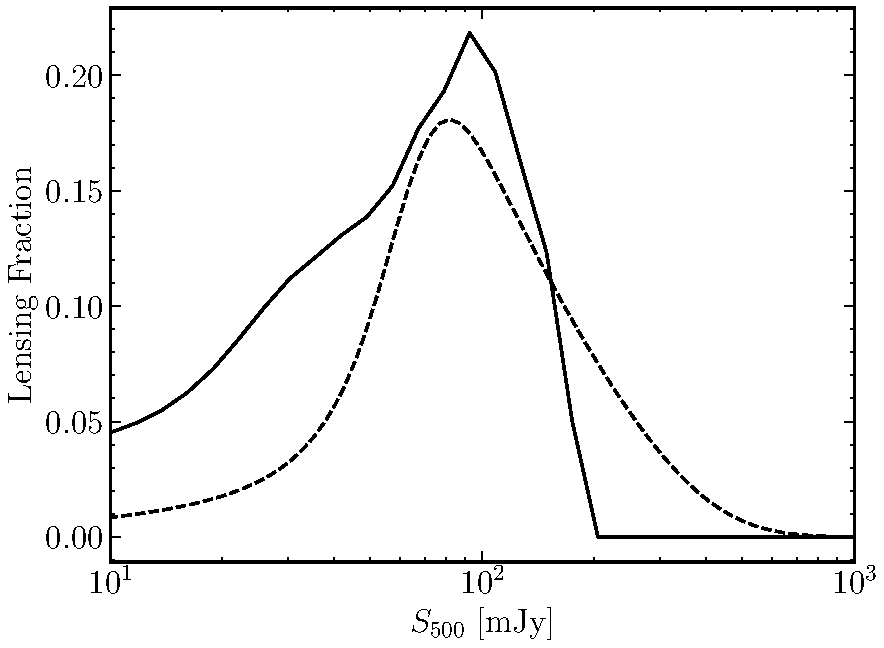
\includegraphics[width=0.5\columnwidth,height=0.24\textheight]{Figures/lensing_fraction.pdf}
    \caption{Top panel: The photometric redshift distribution of \textit{Herschel} sources split into the following categories: the best photometric redshift of all sources (solid black line), the redshift distribution of candidate lensed systems according to $z_{\textrm{sub-mm}}$ (solid red line), and the corresponding redshift distribution of VIKING counterparts (pink solid line). The black and red dashed lines represent the prediction from the \citealt{Cai_2013} evolution model for all sources and lensed sources respectively. Middle panel: The cumulative number counts for candidate lensed systems in the SGP as a function of 500\,\micron flux density (red circles) compared to the samples presented in \citealt{Negrello_2017} (blue circles) and \citealt{Nayyeri_2016} (green circles). The total source counts and lensed counts predicted by the \citealt{Cai_2013} model are shown as dashed black and red lines respectively. Bottom panel: The fraction of sources that are gravitationally lensed in the SGP as a function of 500\,\micron flux density (solid black line), compared with the prediction of \citealt{Cai_2013} (dashed black line).
    \label{fig:lens_distributions_against_cai}}
\end{figure}

\section{The Full \textit{Herschel}-ATLAS Project}
% Include correlations with redshift now they have been described (e.g. flux and magnitude against redshift)
% Include a description of the full H-ATLAS: a legacy product that has no plans for being replaced

\section{Conclusion}